\documentclass[11pt]{article}
\usepackage[margin=2cm]{geometry}
\usepackage{graphicx}
\usepackage{amsmath,amssymb}
\usepackage{xcolor}
\usepackage[hidelinks]{hyperref}
\setlength{\parindent}{0pt}
\begin{document}

\begin{titlepage}
\centering
{\Huge\bfseries Catalogue of Symmetric Graph Drawings\par}
\vspace{1cm}
{\large One page per drawing in \texttt{individual\_graphs/}\par}
\vspace{2cm}
\begin{minipage}{0.8\textwidth}
Each graph was laid out by the orbit-quotient pipeline
(\texttt{src/draw\_graph.py} + \texttt{src/symmetric-layout.g}): GAP computes
$\mathrm{Aut}(\Gamma)$ and an orbit decomposition under a chosen subgroup, and
each orbit is placed on a concentric ring with rotational symmetry. Pages
marked \emph{hand-edited} were tuned manually after generation. Group facts
follow \texttt{docs/CATALOGUE.md}; the research context is in
\texttt{docs/RESEARCH\_PROGRAM.md}.
\end{minipage}
\vfill
{\small Generated by \texttt{src/make\_catalogue.py} --- regenerate after adding drawings.\par}
\end{titlepage}

\tableofcontents
\newpage
\addtocontents{toc}{\protect\vspace{0.5em}\protect\noindent\textbf{Foster Census Classics}\protect\par}
\section{$K_4$ (F004A)}
\begin{center}
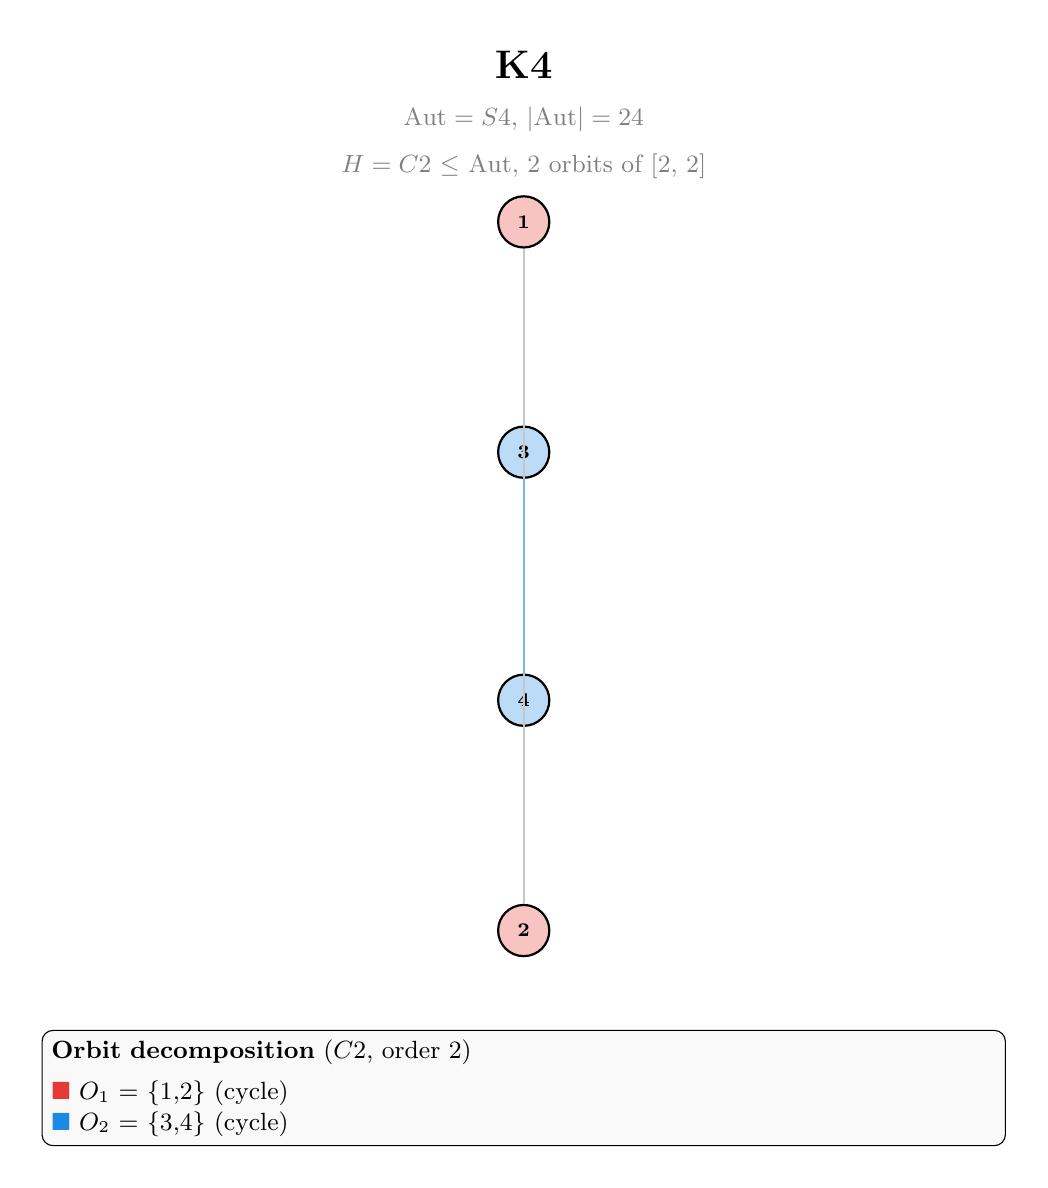
\includegraphics[width=0.92\textwidth,height=0.66\textheight,keepaspectratio]{individual_graphs/auto-k4.jpg}
\end{center}
\vfill
The complete graph on 4 vertices — the tetrahedron skeleton and the smallest cubic arc-transitive graph. $\mathrm{Aut} = S_4$ of order 24.

\medskip
{\small\color{gray}\texttt{individual\_graphs/auto-k4.pdf}}
\newpage
\section{$K_{3,3}$ (F006A)}
\begin{center}
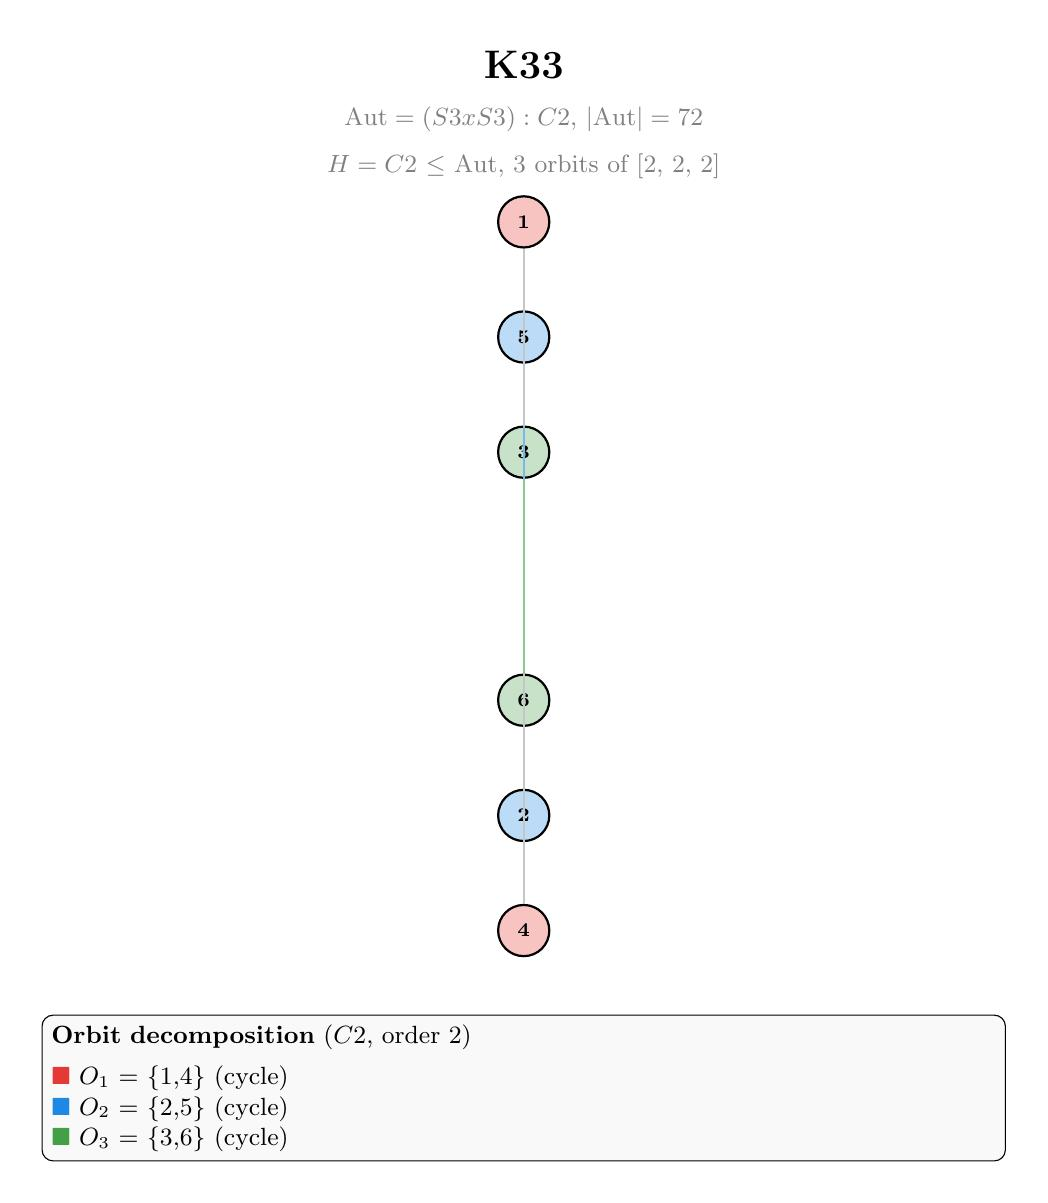
\includegraphics[width=0.92\textwidth,height=0.66\textheight,keepaspectratio]{individual_graphs/auto-k33.jpg}
\end{center}
\vfill
The complete bipartite graph on $3+3$ vertices (the `utility graph'), Levi graph of the degenerate digon geometry. $\mathrm{Aut} = (S_3 \times S_3) \rtimes C_2$ of order 72.

\medskip
{\small\color{gray}\texttt{individual\_graphs/auto-k33.pdf}}
\newpage
\section{Cube $Q_3$ = GP(4,1) (F008A)}
\begin{center}
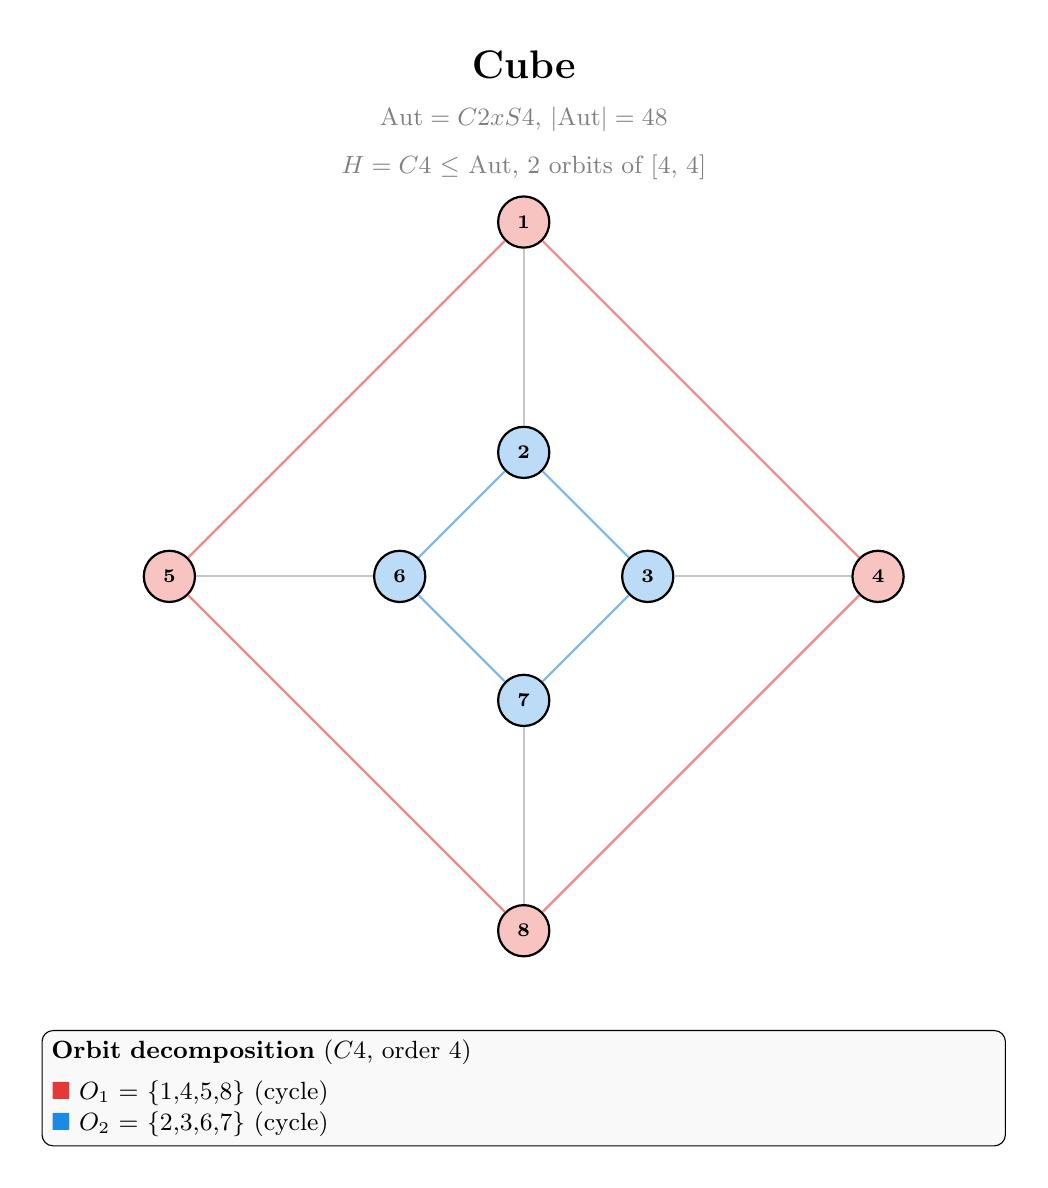
\includegraphics[width=0.92\textwidth,height=0.66\textheight,keepaspectratio]{individual_graphs/auto-cube.jpg}
\end{center}
\vfill
The 3-dimensional hypercube on 8 vertices, drawn as two concentric 4-rings. $\mathrm{Aut} = C_2 \times S_4$ of order 48.

\medskip
{\small\color{gray}\texttt{individual\_graphs/auto-cube.pdf}}
\newpage
\section{Petersen = GP(5,2) (F010A)}
\begin{center}
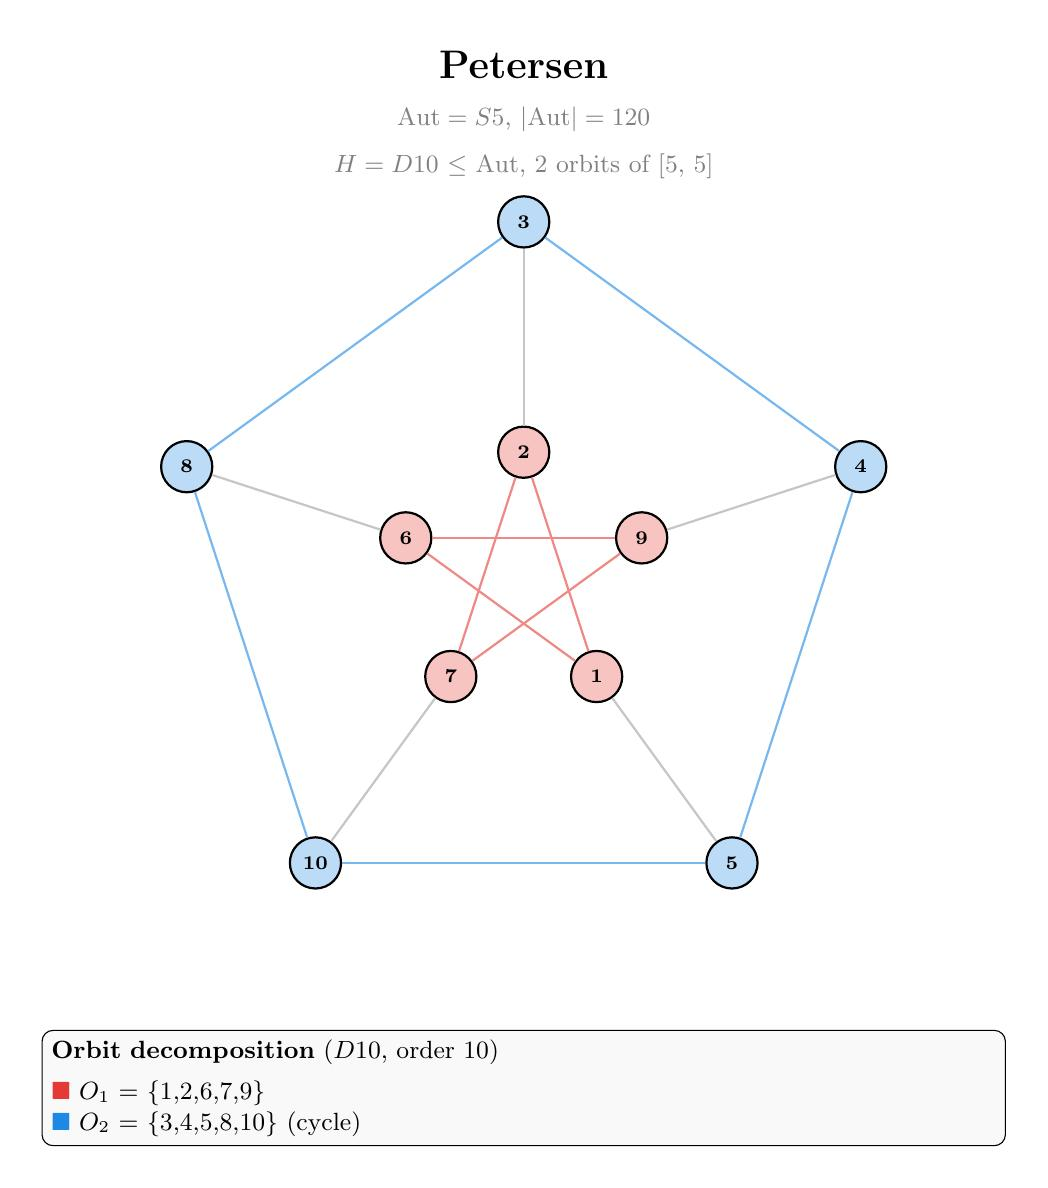
\includegraphics[width=0.92\textwidth,height=0.66\textheight,keepaspectratio]{individual_graphs/auto-petersen.jpg}
\end{center}
\vfill
The Petersen graph on 10 vertices: Kneser graph $K(5,2)$, $\mathrm{Aut} = S_5 \cong \mathrm{PGL}(2,5)$ of order 120. Drawn on two $D_{10}$-orbit rings of 5 — the classic pentagon/pentagram picture.

\medskip
{\small\color{gray}\texttt{individual\_graphs/auto-petersen.pdf}}
\newpage
\section{Heawood (F014A)}
\begin{center}
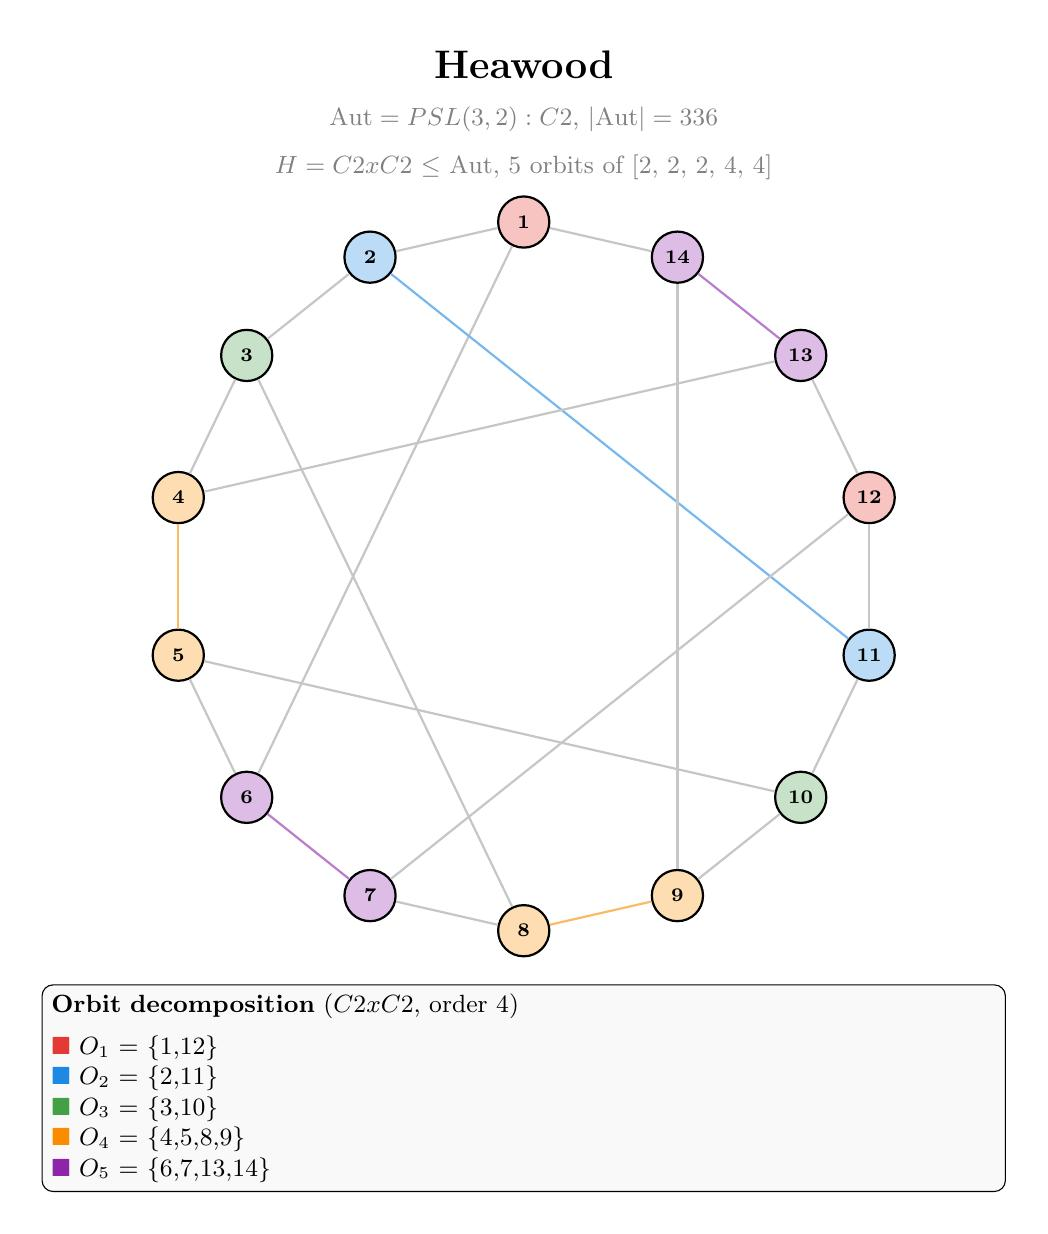
\includegraphics[width=0.92\textwidth,height=0.66\textheight,keepaspectratio]{individual_graphs/auto-heawood.jpg}
\end{center}
\vfill
The Heawood graph on 14 vertices: Levi (point--line incidence) graph of the Fano plane $\mathrm{PG}(2,2)$ and the $(3,6)$-cage. $\mathrm{Aut} = \mathrm{PGL}(2,7)$ of order 336.

\medskip
{\small\color{gray}\texttt{individual\_graphs/auto-heawood.pdf}}
\newpage
\section{M\"obius--Kantor = GP(8,3) (F016A)}
\begin{center}
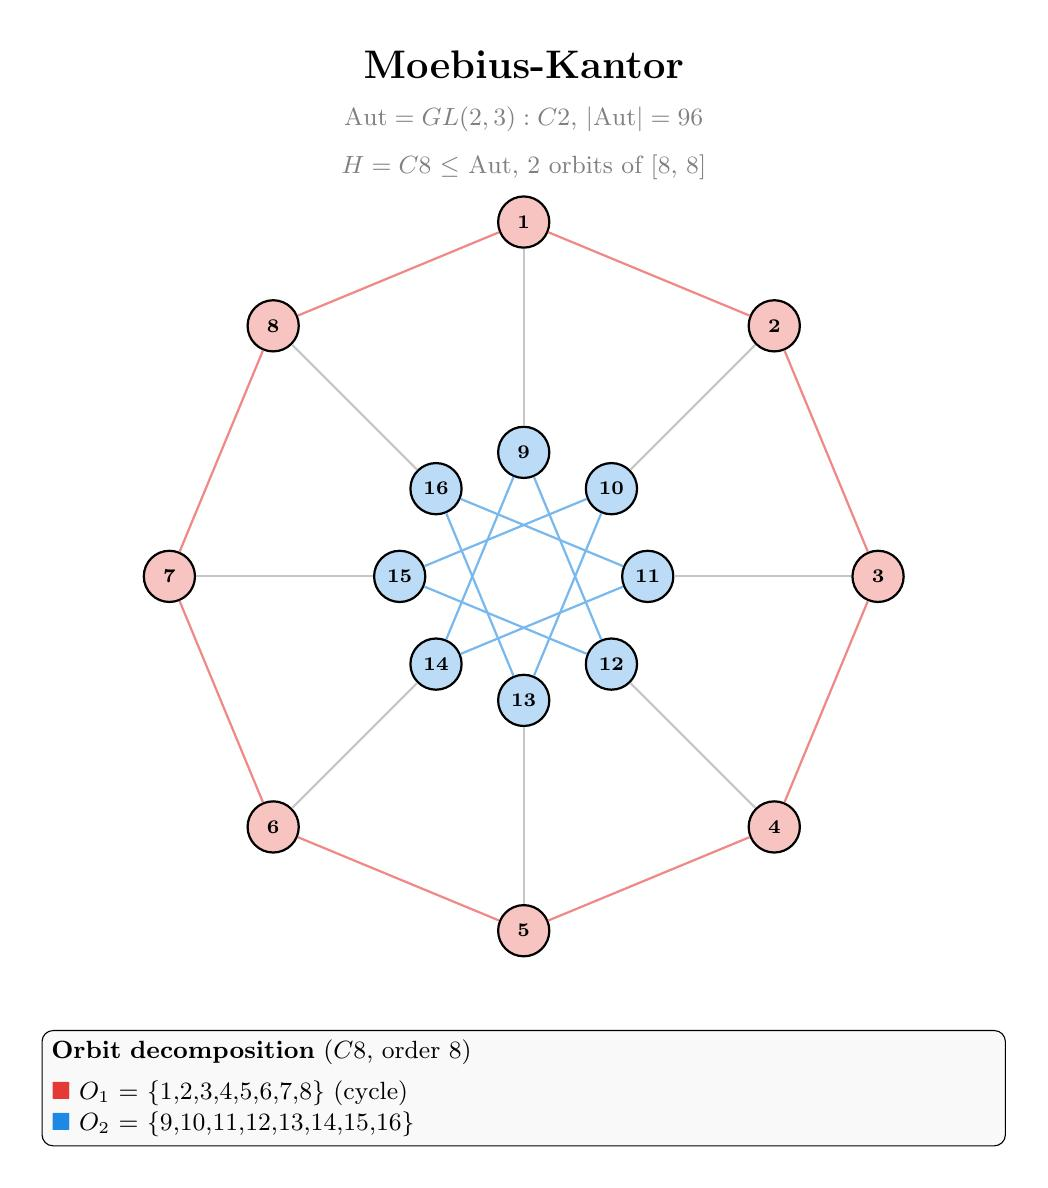
\includegraphics[width=0.92\textwidth,height=0.66\textheight,keepaspectratio]{individual_graphs/auto-moebiuskantor.jpg}
\end{center}
\vfill
The M\"obius--Kantor graph on 16 vertices, generalized Petersen $\mathrm{GP}(8,3)$, drawn on two $C_8$-orbit rings. $\mathrm{Aut} = \mathrm{GL}(2,3) \rtimes C_2$ of order 96.

\medskip
{\small\color{gray}\texttt{individual\_graphs/auto-moebiuskantor.pdf}}
\newpage
\section{Pappus (F018A)}
\begin{center}
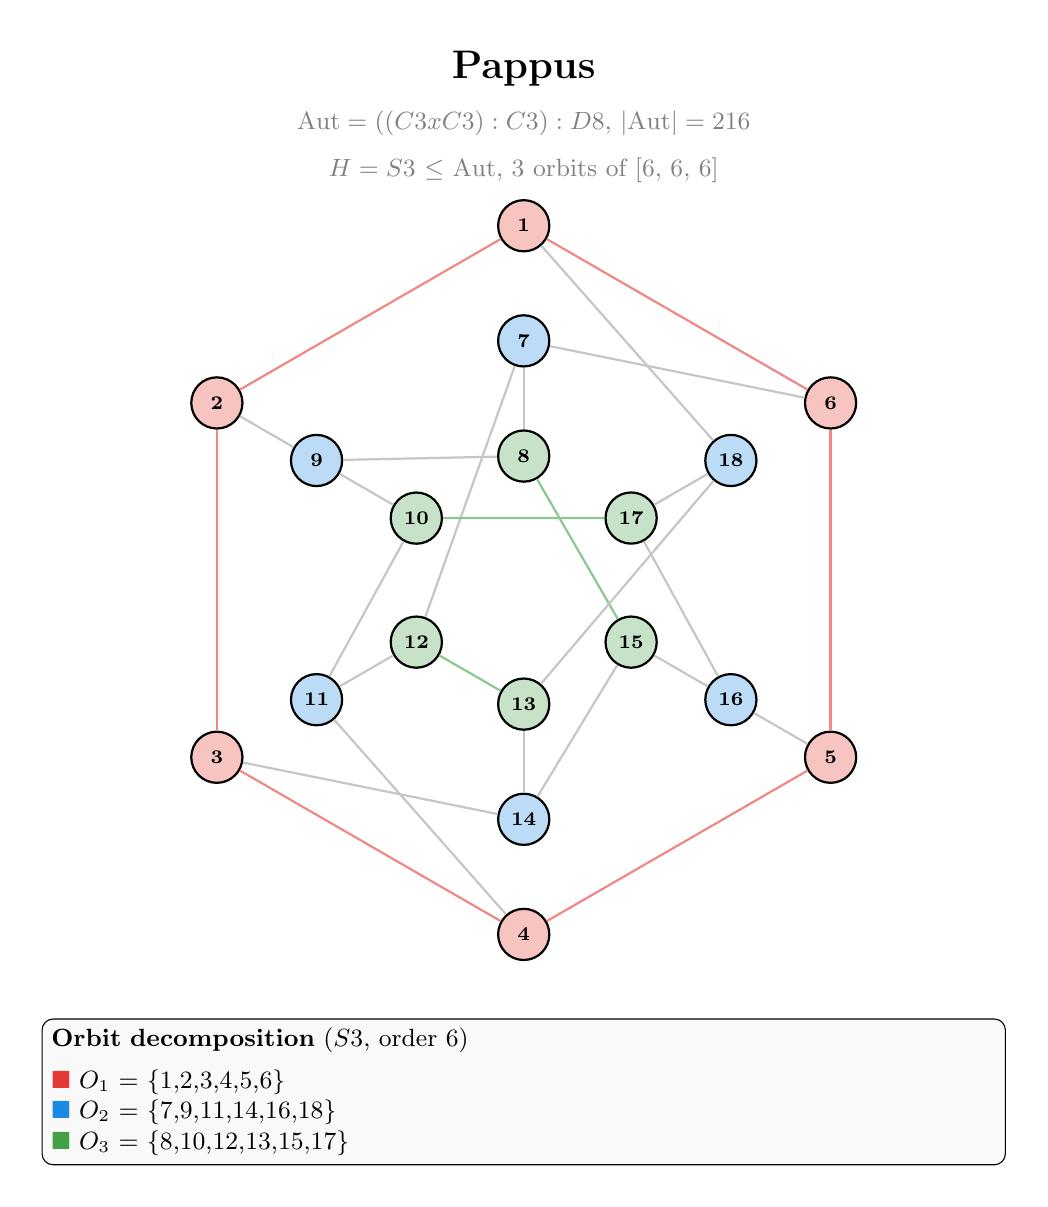
\includegraphics[width=0.92\textwidth,height=0.66\textheight,keepaspectratio]{individual_graphs/auto-pappus.jpg}
\end{center}
\vfill
The Pappus graph on 18 vertices: Levi graph of the Pappus configuration $(9_3, 9_3)$, tied to the affine plane $\mathrm{AG}(2,3)$. $\mathrm{Aut}$ has order 216; drawn as three $S_3$-orbit rings of 6.

\medskip
{\small\color{gray}\texttt{individual\_graphs/auto-pappus.pdf}}
\newpage
\section{Desargues = GP(10,3) (F020A)}
\begin{center}
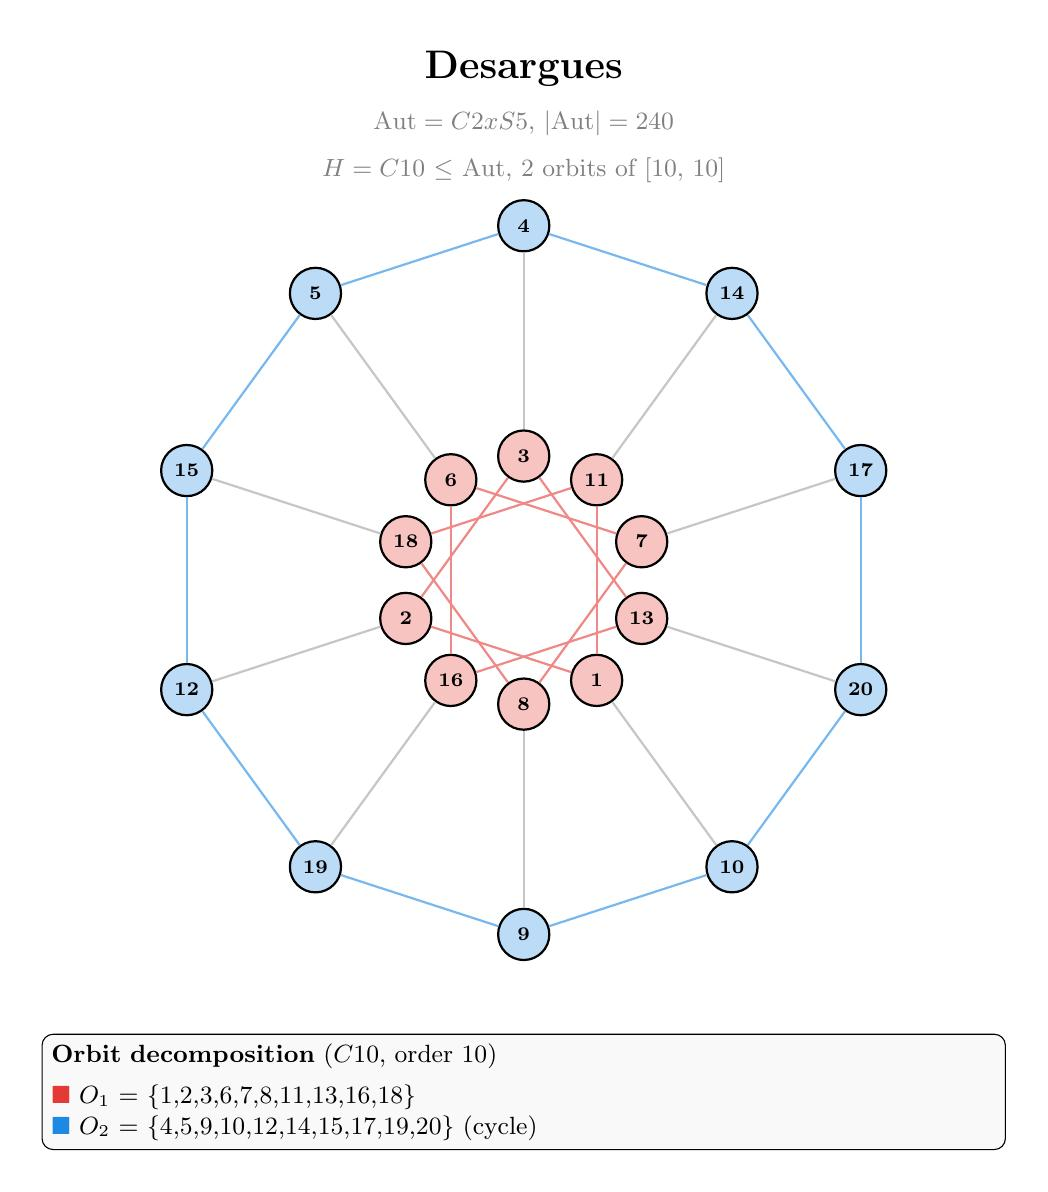
\includegraphics[width=0.92\textwidth,height=0.66\textheight,keepaspectratio]{individual_graphs/auto-desargues.jpg}
\end{center}
\vfill
The Desargues graph on 20 vertices: Levi graph of the Desargues configuration $(10_3, 10_3)$. $\mathrm{Aut} = C_2 \times S_5$ of order 240; two $C_{10}$-orbit rings of 10.

\medskip
{\small\color{gray}\texttt{individual\_graphs/auto-desargues.pdf}}
\newpage
\section{Dodecahedron (F020B)}
\begin{center}
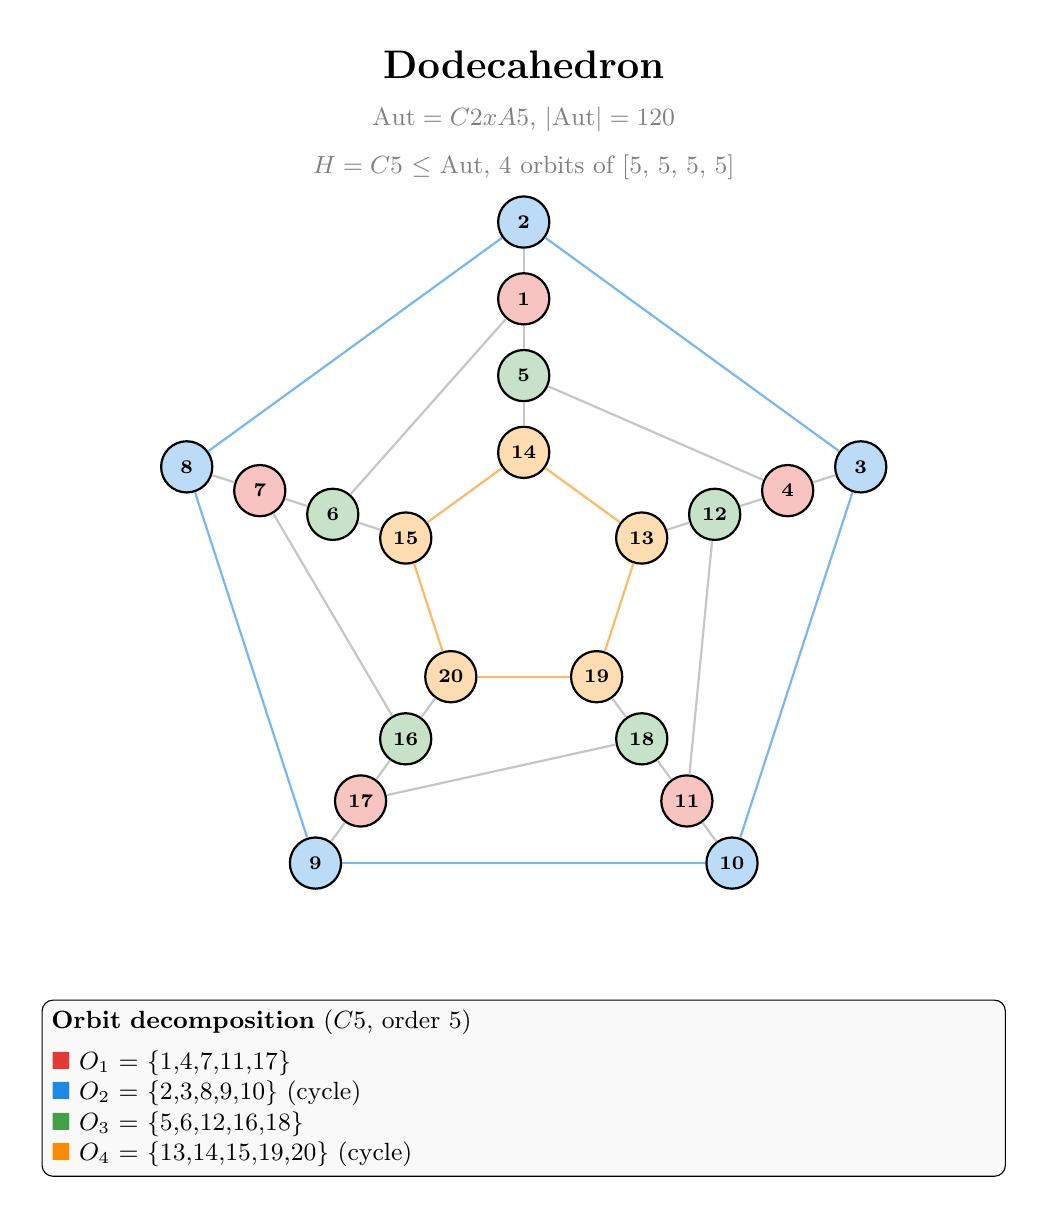
\includegraphics[width=0.92\textwidth,height=0.66\textheight,keepaspectratio]{individual_graphs/auto-dodecahedron.jpg}
\end{center}
\vfill
The skeleton of the regular dodecahedron, 20 vertices. $\mathrm{Aut} = C_2 \times A_5$ of order 120; four $C_5$-orbit rings of 5 give the Schlegel-like layout.

\medskip
{\small\color{gray}\texttt{individual\_graphs/auto-dodecahedron.pdf}}
\newpage
\section{Nauru = GP(12,5) (F024A)}
\begin{center}
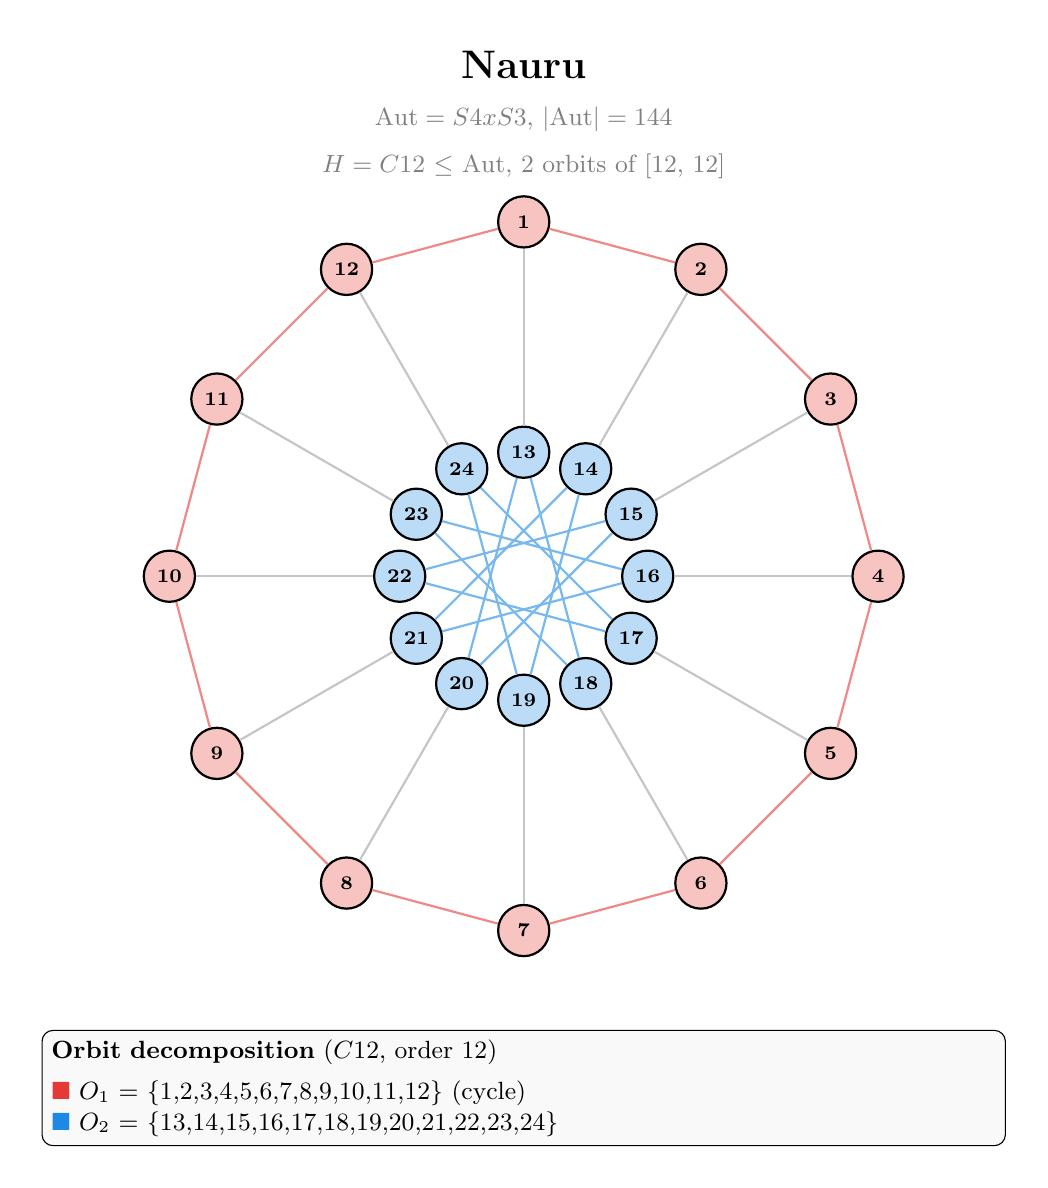
\includegraphics[width=0.92\textwidth,height=0.66\textheight,keepaspectratio]{individual_graphs/auto-nauru.jpg}
\end{center}
\vfill
The Nauru graph on 24 vertices, generalized Petersen $\mathrm{GP}(12,5)$. $\mathrm{Aut} = S_4 \times S_3$ of order 144; two $C_{12}$-orbit rings of 12.

\medskip
{\small\color{gray}\texttt{individual\_graphs/auto-nauru.pdf}}
\newpage
\section{$F_{26A}$}
\begin{center}
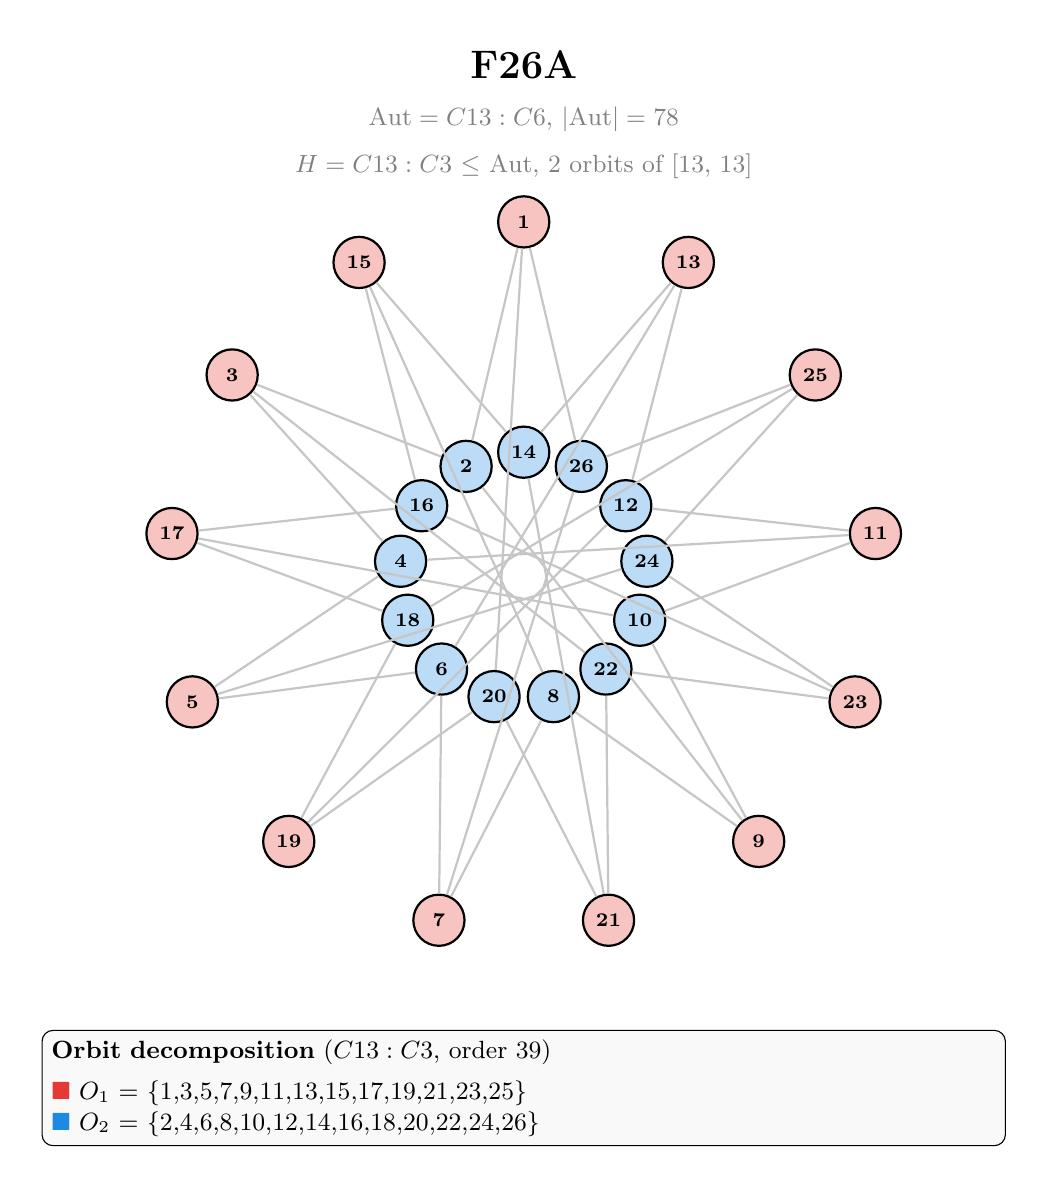
\includegraphics[width=0.92\textwidth,height=0.66\textheight,keepaspectratio]{individual_graphs/auto-f26a.jpg}
\end{center}
\vfill
The F26A graph on 26 vertices, $\mathrm{Aut} = C_{13} \rtimes C_6$ of order 78 — the smallest Foster-census entry whose full automorphism group is solvable of this metacyclic shape. Two rings of 13.

\medskip
{\small\color{gray}\texttt{individual\_graphs/auto-f26a.pdf}}
\newpage
\section{Coxeter (F028A)}
\begin{center}
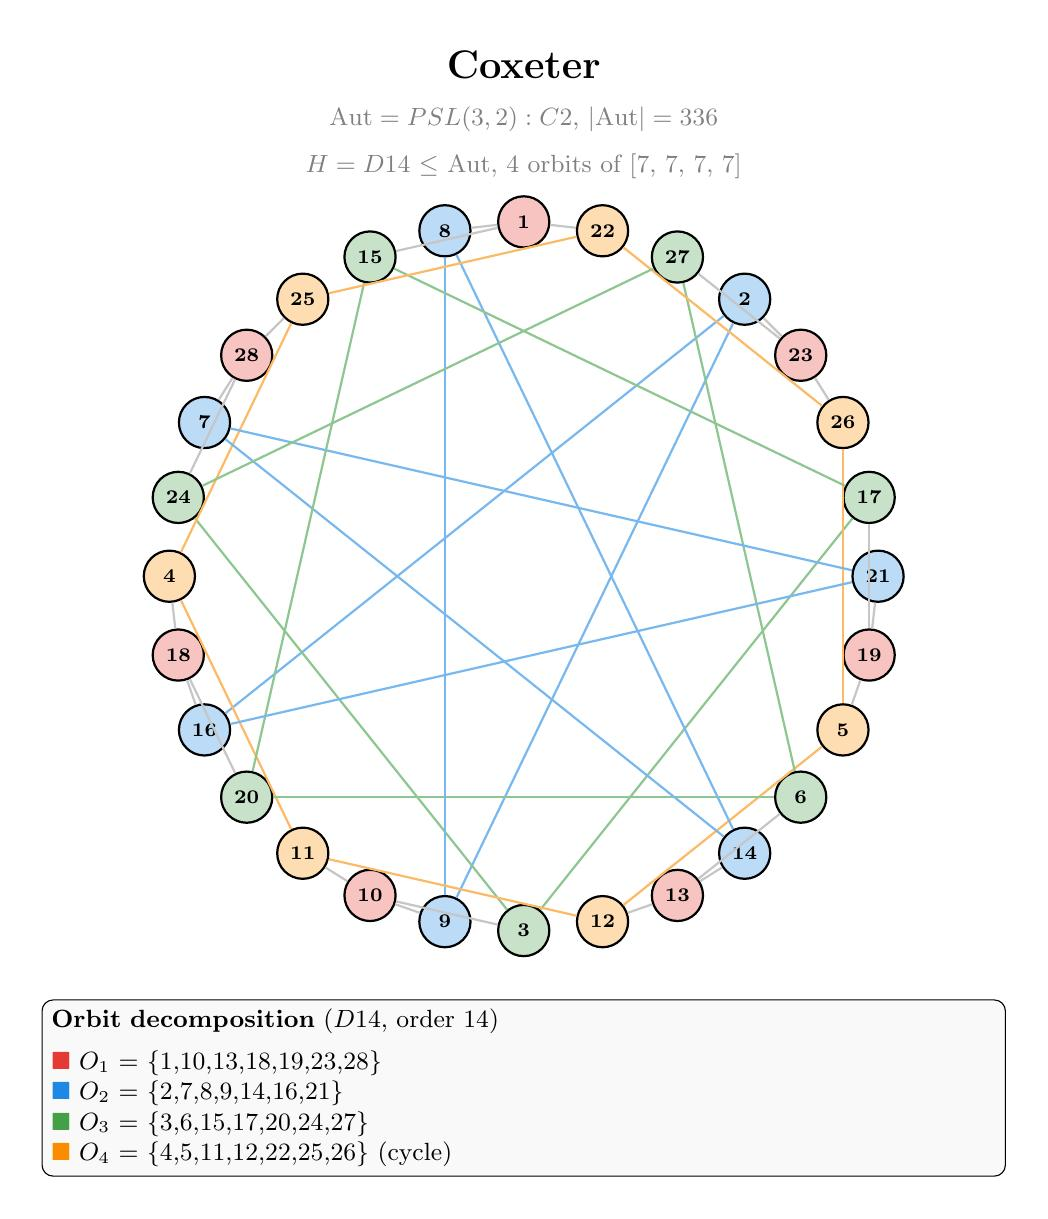
\includegraphics[width=0.92\textwidth,height=0.66\textheight,keepaspectratio]{individual_graphs/auto-coxeter.jpg}
\end{center}
\vfill
The Coxeter graph on 28 vertices, a famous non-hamiltonian cubic graph. $\mathrm{Aut} = \mathrm{PGL}(2,7)$ of order 336 (the same group as Heawood); four $D_{14}$-orbit rings of 7.

\medskip
{\small\color{gray}\texttt{individual\_graphs/auto-coxeter.pdf}}
\newpage
\section{Tutte--Coxeter (F030A)}
\begin{center}
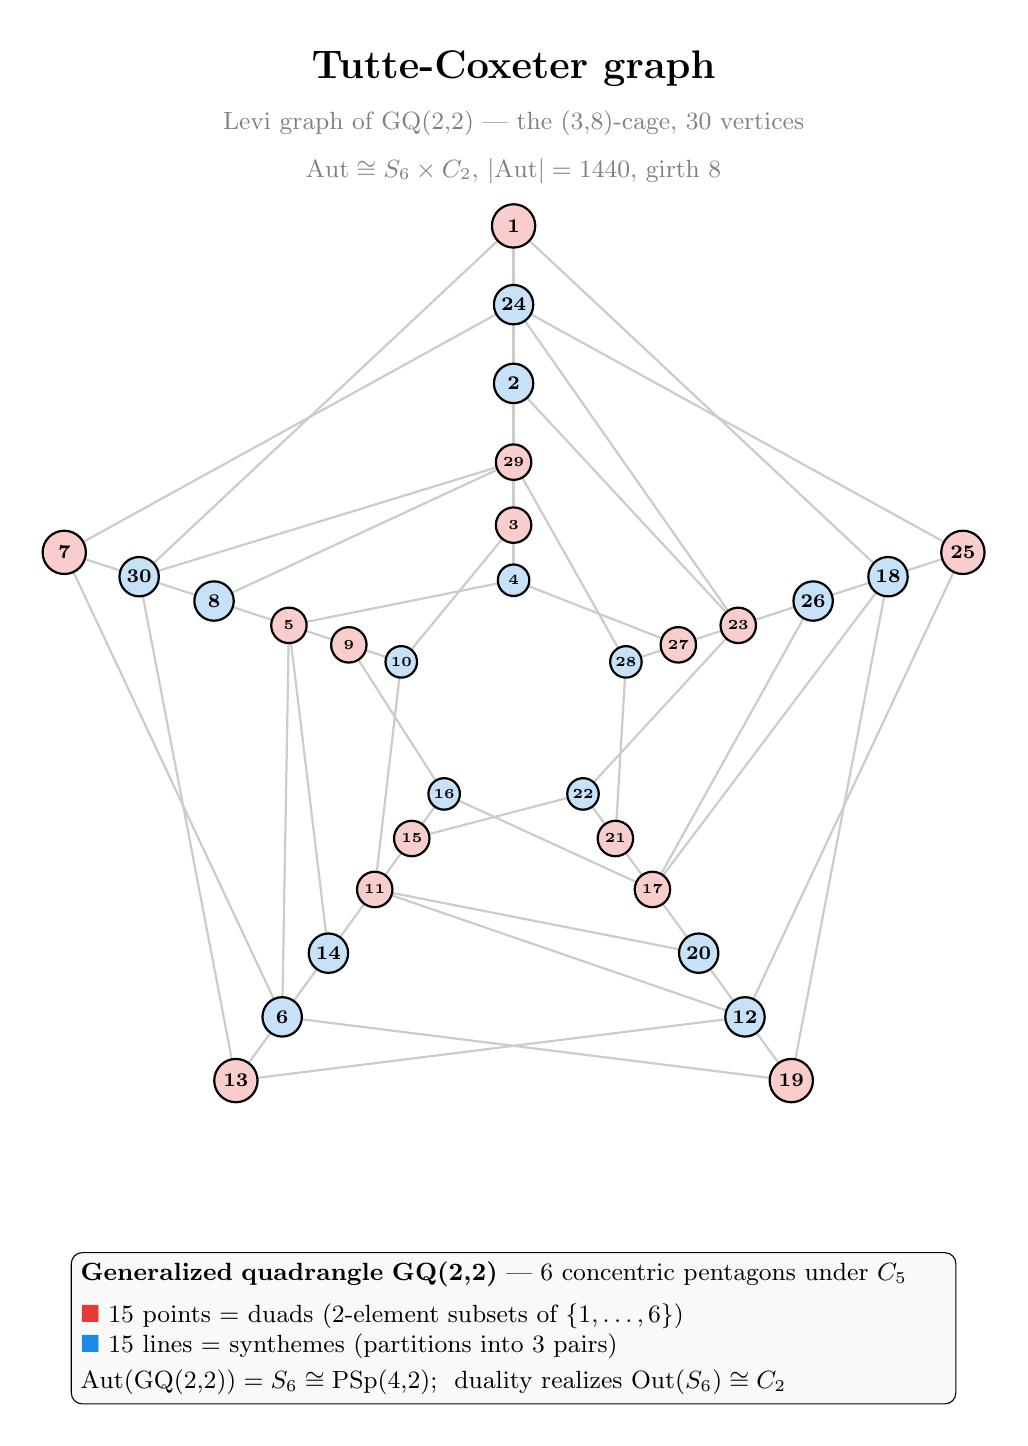
\includegraphics[width=0.92\textwidth,height=0.66\textheight,keepaspectratio]{individual_graphs/auto-tuttecoxeter.jpg}
\end{center}
\vfill
The Tutte--Coxeter graph on 30 vertices: Levi graph of the generalized quadrangle $\mathrm{GQ}(2,2)$ and the $(3,8)$-cage. $\mathrm{Aut} \cong \mathrm{Aut}(S_6)$ of order 1440 — the home of $S_6$'s outer automorphism. Three rings of 10.

\medskip
{\small\color{gray}\texttt{individual\_graphs/auto-tuttecoxeter.pdf}}
\newpage
\addtocontents{toc}{\protect\vspace{0.5em}\protect\noindent\textbf{PSL(2,q) Family}\protect\par}
\section{$\mathrm{PSL}(2,5)/C_3$ — double cover of Petersen}
\begin{center}
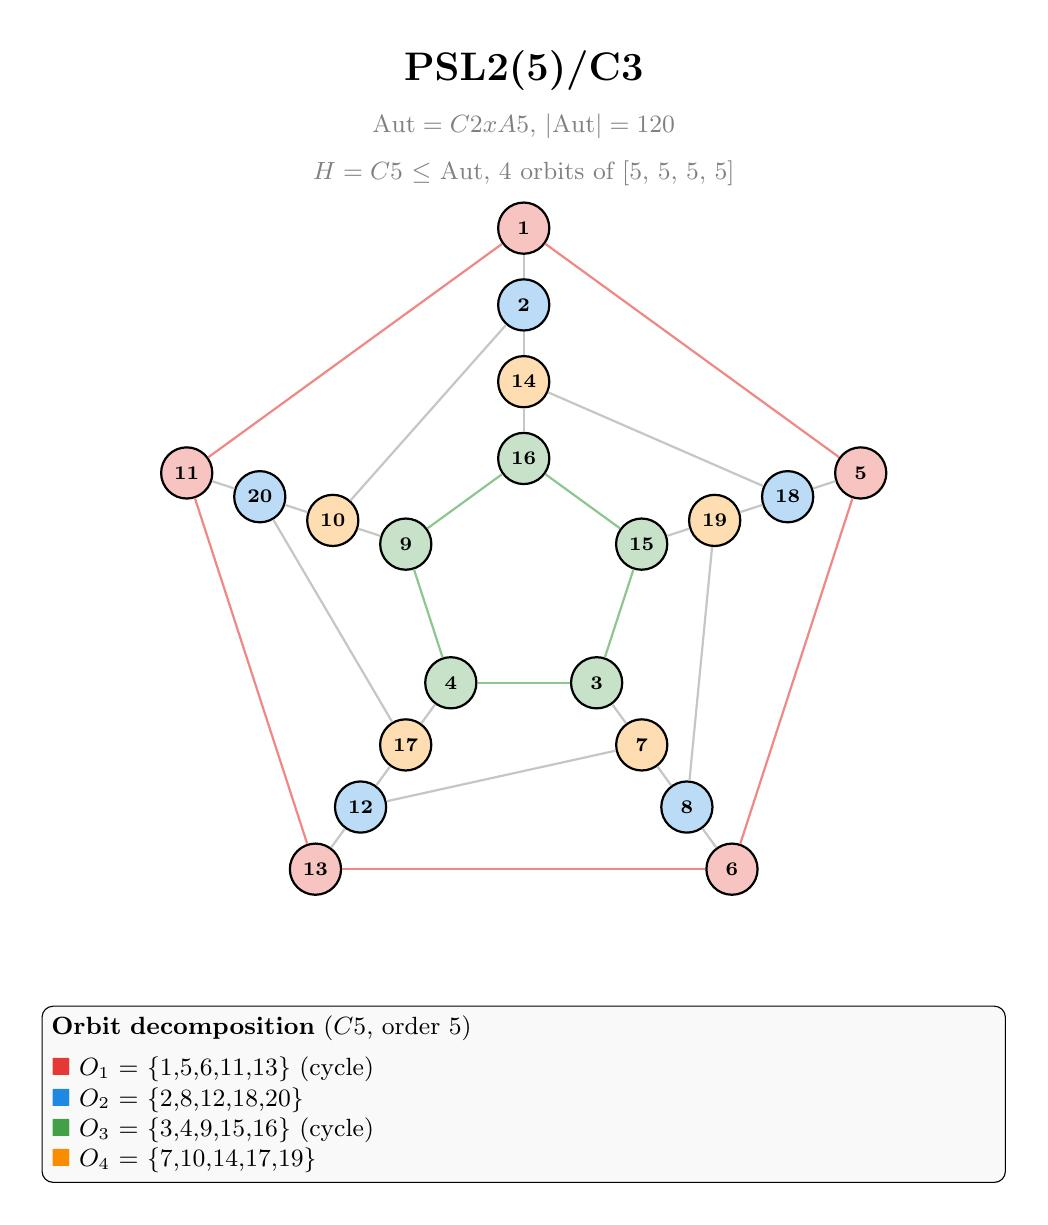
\includegraphics[width=0.92\textwidth,height=0.66\textheight,keepaspectratio]{individual_graphs/auto-psl2_5_c3.jpg}
\end{center}
\vfill
Coset graph of $\mathrm{PSL}(2,5) \cong A_5$ on the 20 cosets of a $C_3$ point stabilizer: a double cover of the Petersen graph. First rung of the $C_3 \subset S_3 \subset S_4$ tower of covers.

\medskip
{\small\color{gray}\texttt{individual\_graphs/auto-psl2\_5\_c3.pdf}}
\newpage
\section{$\mathrm{PSL}(2,7)/C_3$ — 56-vertex coset graph}
\begin{center}
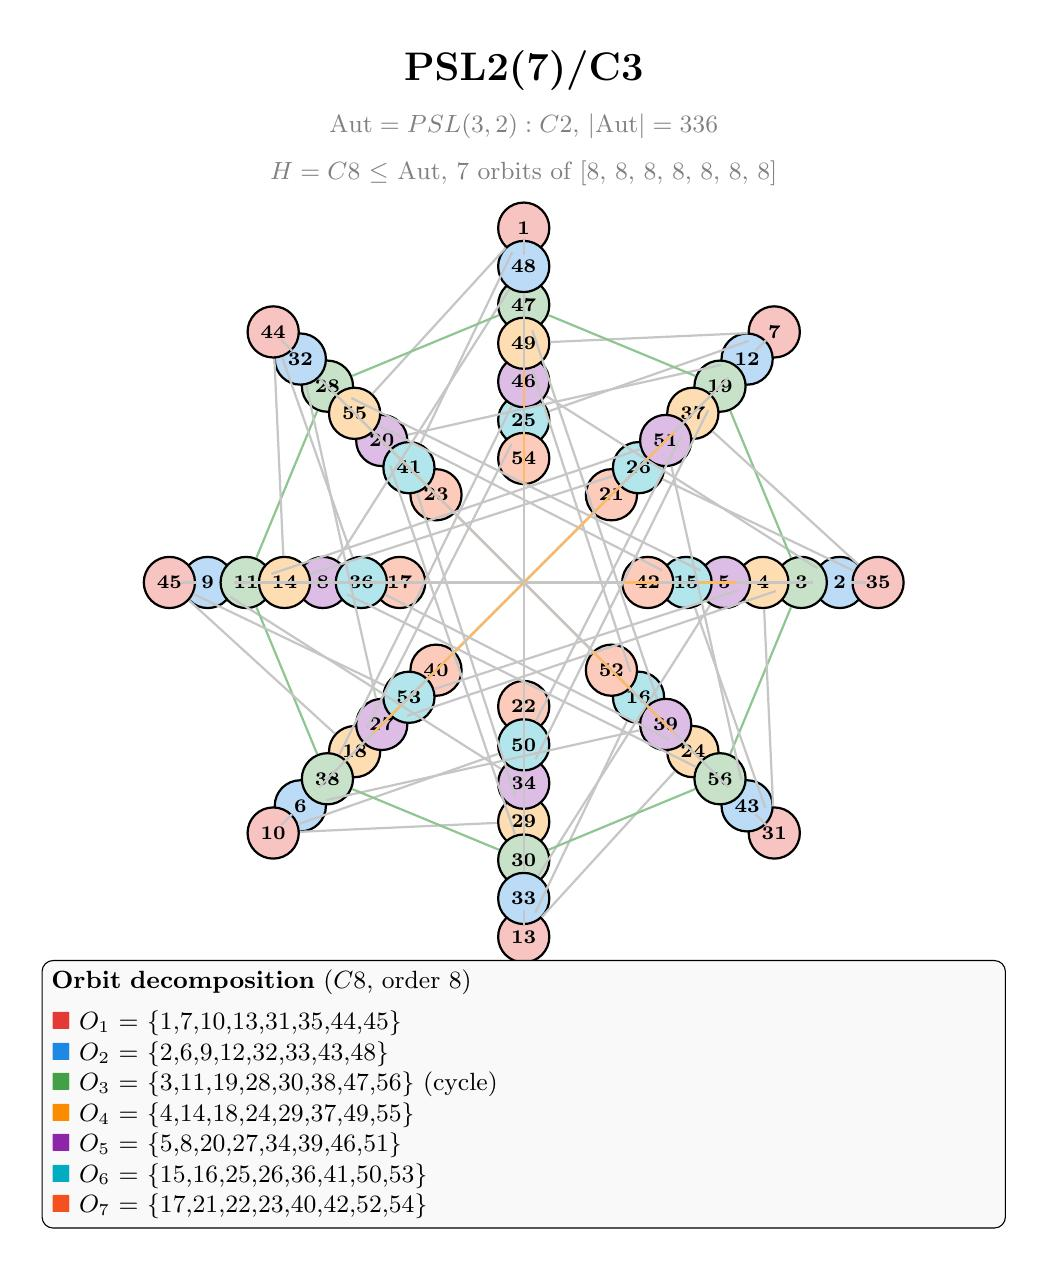
\includegraphics[width=0.92\textwidth,height=0.66\textheight,keepaspectratio]{individual_graphs/auto-psl2_7_c3.jpg}
\end{center}
\vfill
Cubic coset graph of $\mathrm{PSL}(2,7)$ (order 168) acting on the 56 cosets of a $C_3$ stabilizer, from the PSL(2,q) census programme.

\medskip
{\small\color{gray}\texttt{individual\_graphs/auto-psl2\_7\_c3.pdf}}
\newpage
\section{$\mathrm{PSL}(2,13)/S_3$ coset graph}
\begin{center}
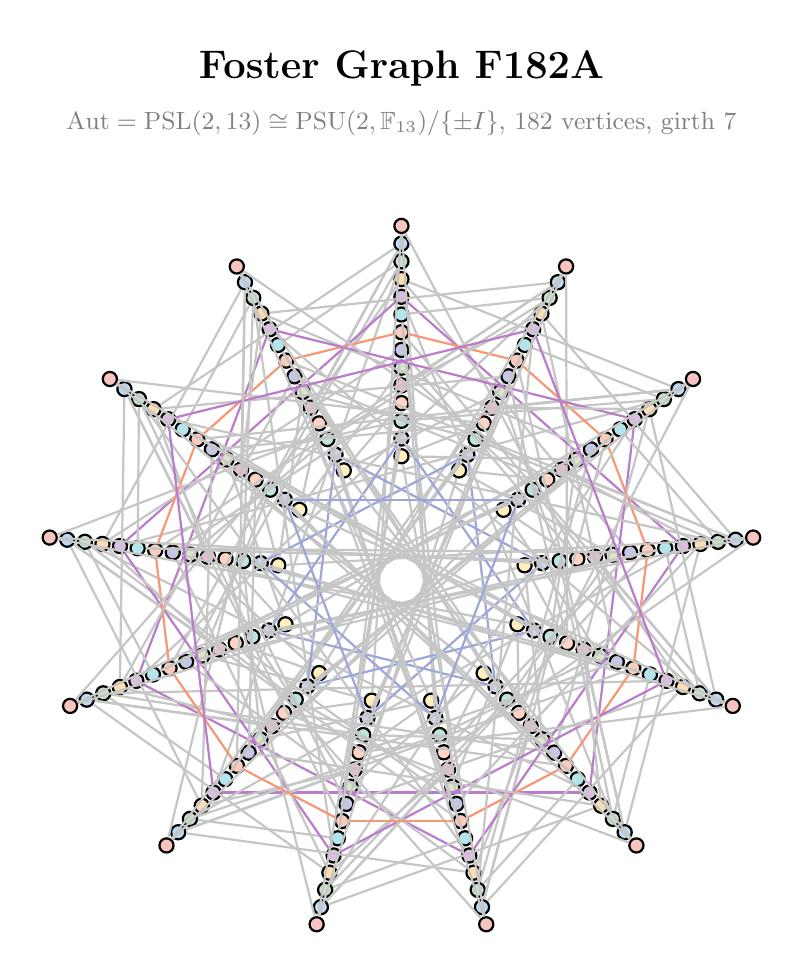
\includegraphics[width=0.92\textwidth,height=0.66\textheight,keepaspectratio]{individual_graphs/auto-psl2_13.jpg}
\end{center}
\vfill
Cubic coset graph of $\mathrm{PSL}(2,13)$ with $S_3$ point stabilizer (the Foster-182 line of the census). Part of the evidence that the $S_3$-stabilizer family is Ramanujan.

\medskip
{\small\color{gray}\texttt{individual\_graphs/auto-psl2\_13.pdf}}
\newpage
\section{Biggs--Smith (F102A)}
\begin{center}
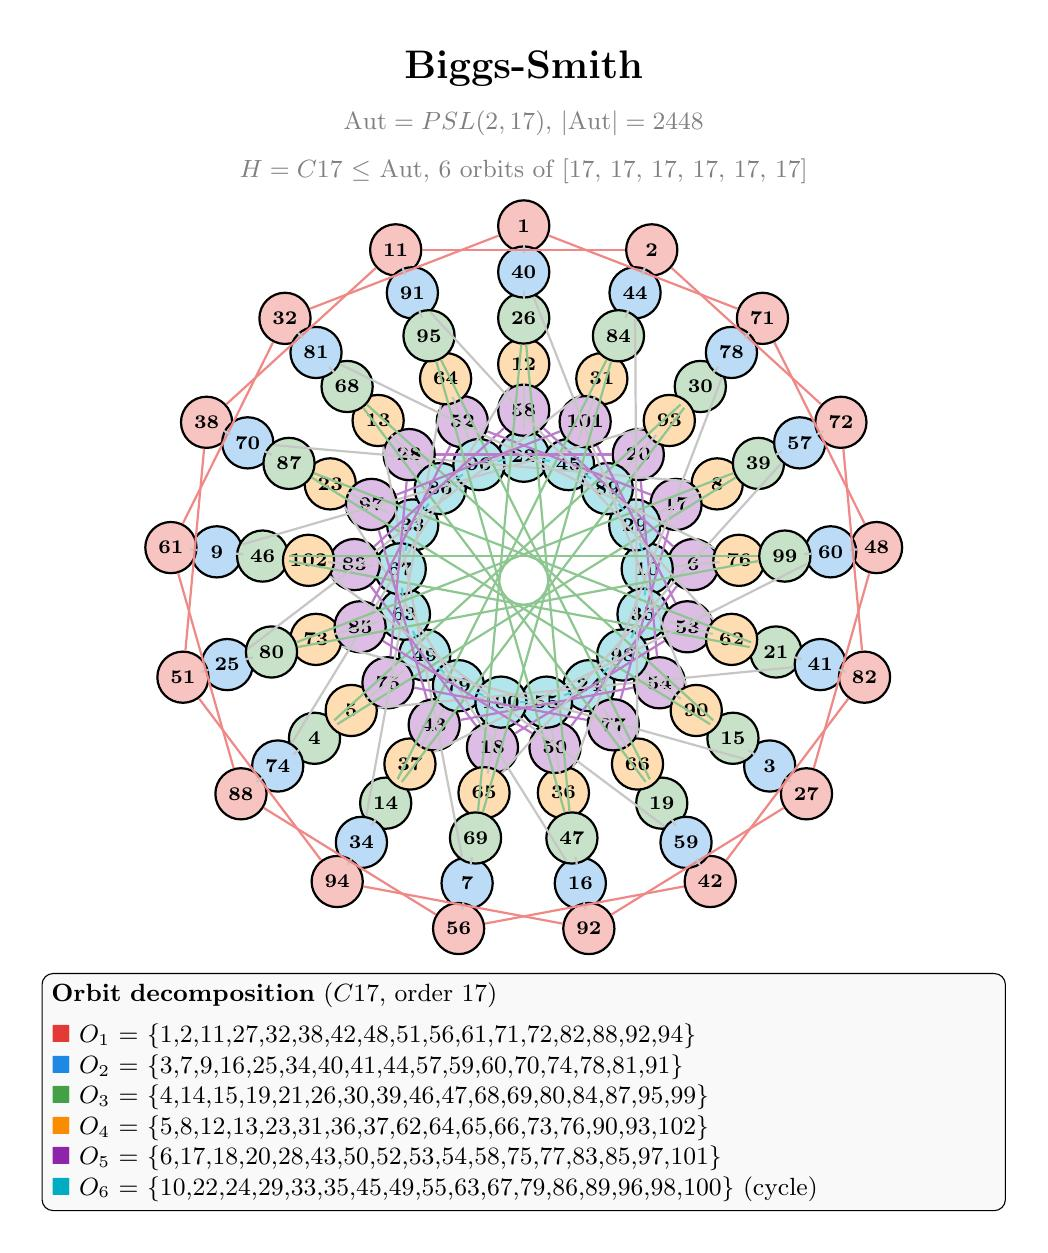
\includegraphics[width=0.92\textwidth,height=0.66\textheight,keepaspectratio]{individual_graphs/auto-biggssmith.jpg}
\end{center}
\vfill
The Biggs--Smith graph on 102 vertices, $\mathrm{Aut} = \mathrm{PSL}(2,17)$ with $S_4$ stabilizer — distance-transitive, and in this programme's slogan ``a picture of $SU(2)$ over $\mathbb{F}_{17}$'' (see docs/RESEARCH\_PROGRAM.md).

\medskip
{\small\color{gray}\texttt{individual\_graphs/auto-biggssmith.pdf}}
\newpage
\section{Biggs--Smith — alternative layout}
\begin{center}
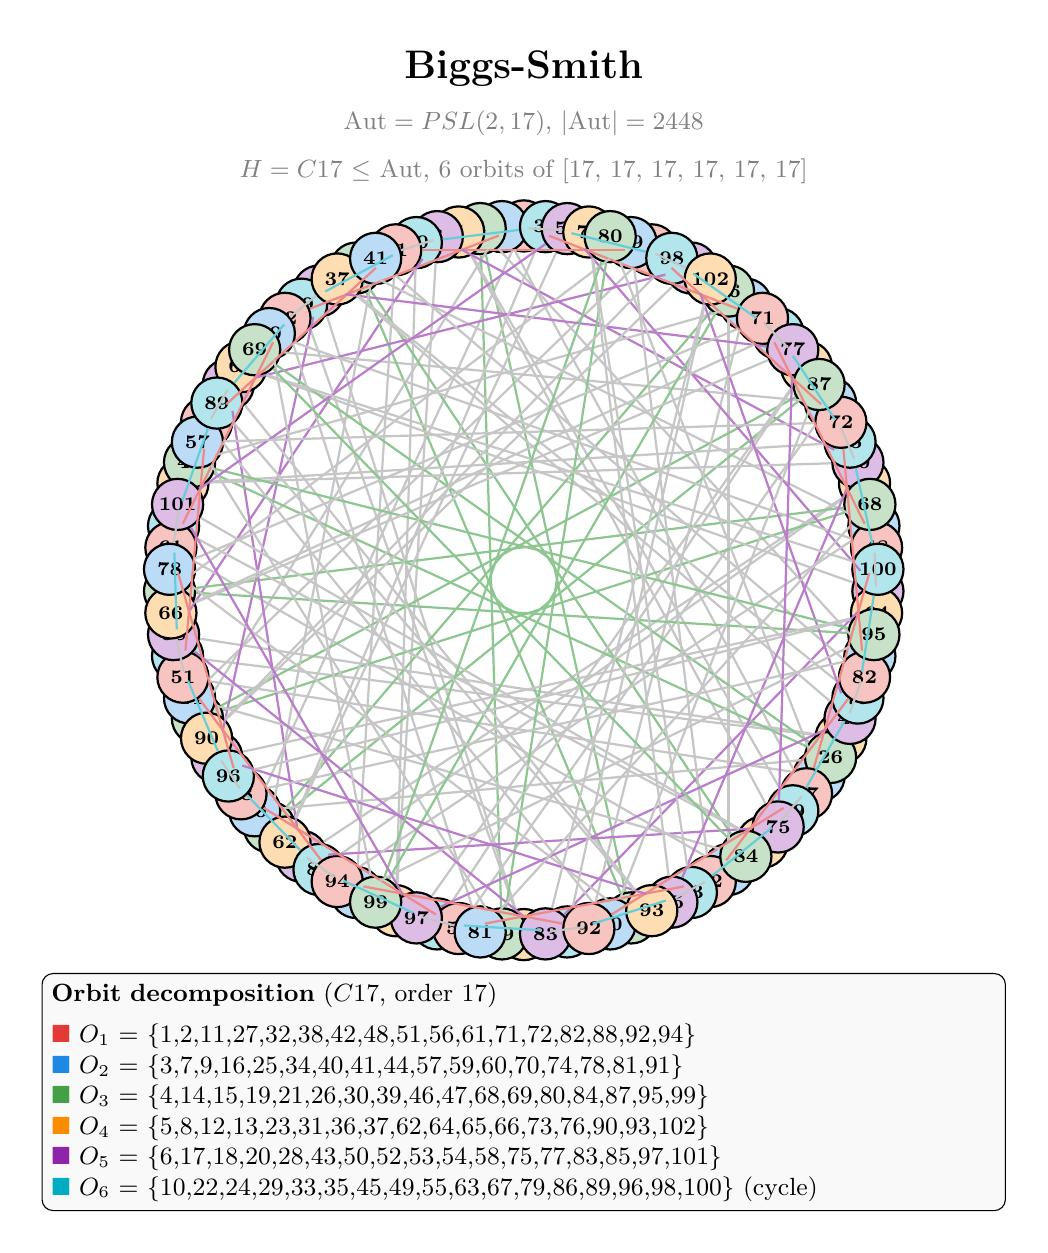
\includegraphics[width=0.92\textwidth,height=0.66\textheight,keepaspectratio]{individual_graphs/auto-biggssmith2.jpg}
\end{center}
\vfill
A second rendering of the Biggs--Smith graph with a different orbit quotient choice, for comparison with the previous page.

\medskip
{\small\color{gray}\texttt{individual\_graphs/auto-biggssmith2.pdf}}
\newpage
\section{Cubic Ramanujan graph from $\mathrm{PSL}(2,19)$}
\begin{center}
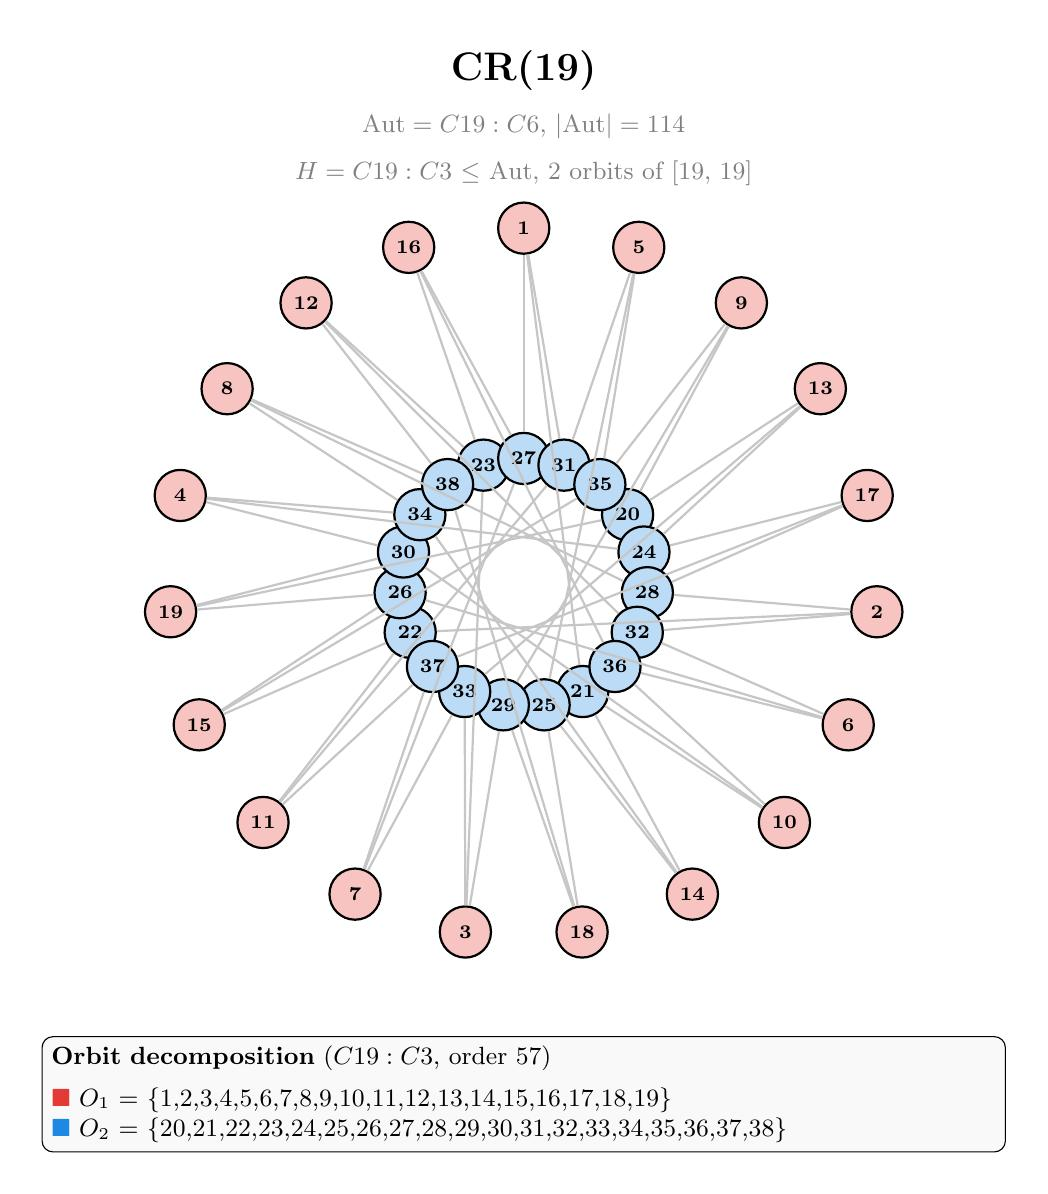
\includegraphics[width=0.92\textwidth,height=0.66\textheight,keepaspectratio]{individual_graphs/auto-cr19.jpg}
\end{center}
\vfill
A cubic Ramanujan graph constructed from $\mathrm{PSL}(2,19)$ in the census programme; spectral bounds checked in src/spectral\_analysis.py.

\medskip
{\small\color{gray}\texttt{individual\_graphs/auto-cr19.pdf}}
\newpage
\section{Cubic Ramanujan graph from $\mathrm{PSL}(2,31)$}
\begin{center}
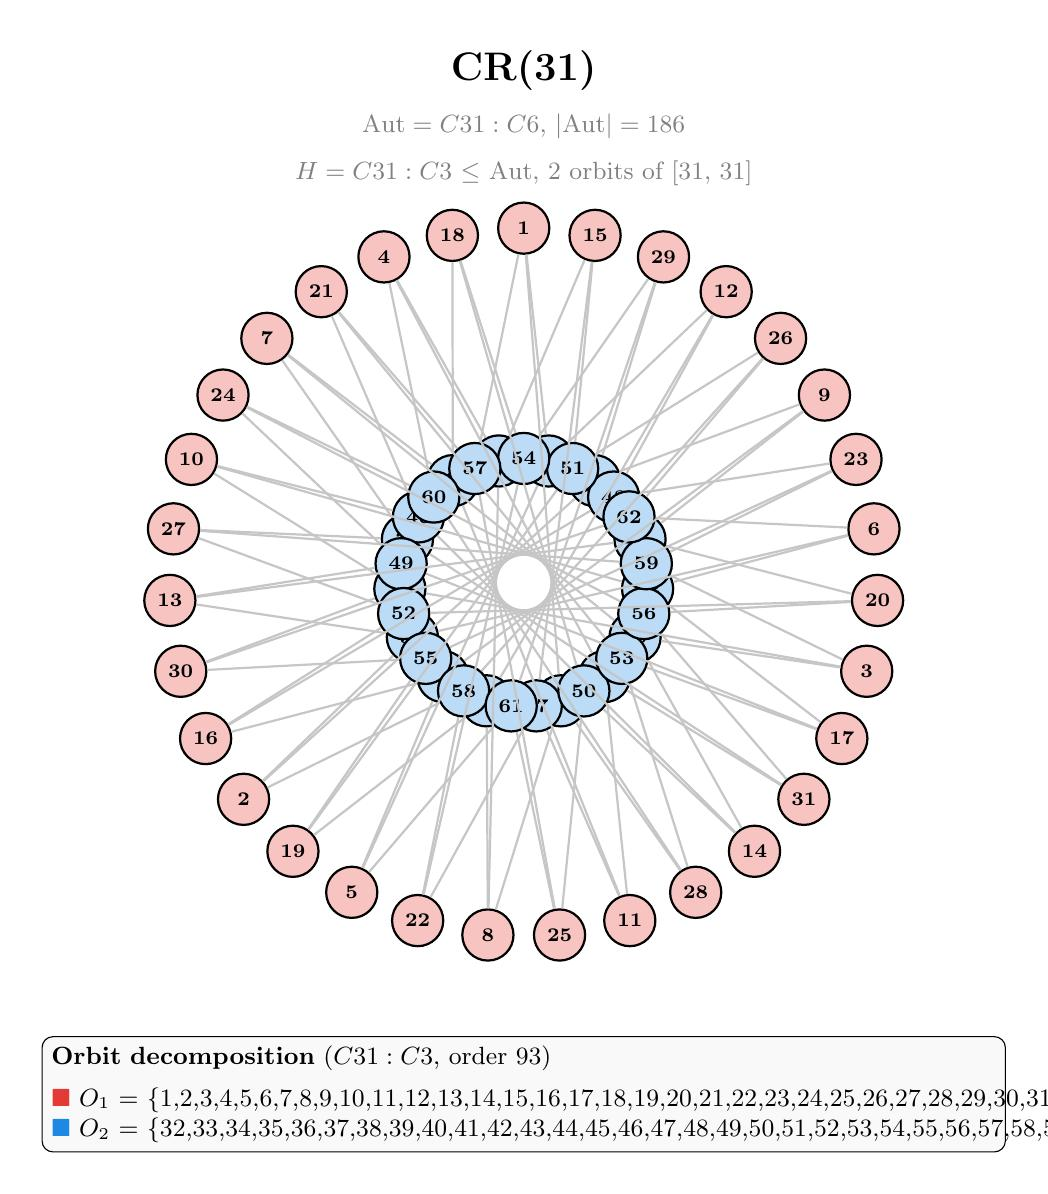
\includegraphics[width=0.92\textwidth,height=0.66\textheight,keepaspectratio]{individual_graphs/auto-cr31.jpg}
\end{center}
\vfill
A cubic Ramanujan graph constructed from $\mathrm{PSL}(2,31)$ — the largest member of the rendered Ramanujan series.

\medskip
{\small\color{gray}\texttt{individual\_graphs/auto-cr31.pdf}}
\newpage
\addtocontents{toc}{\protect\vspace{0.5em}\protect\noindent\textbf{Incidence Geometries}\protect\par}
\section{Levi graph of $\mathrm{PG}(2,3)$}
\begin{center}
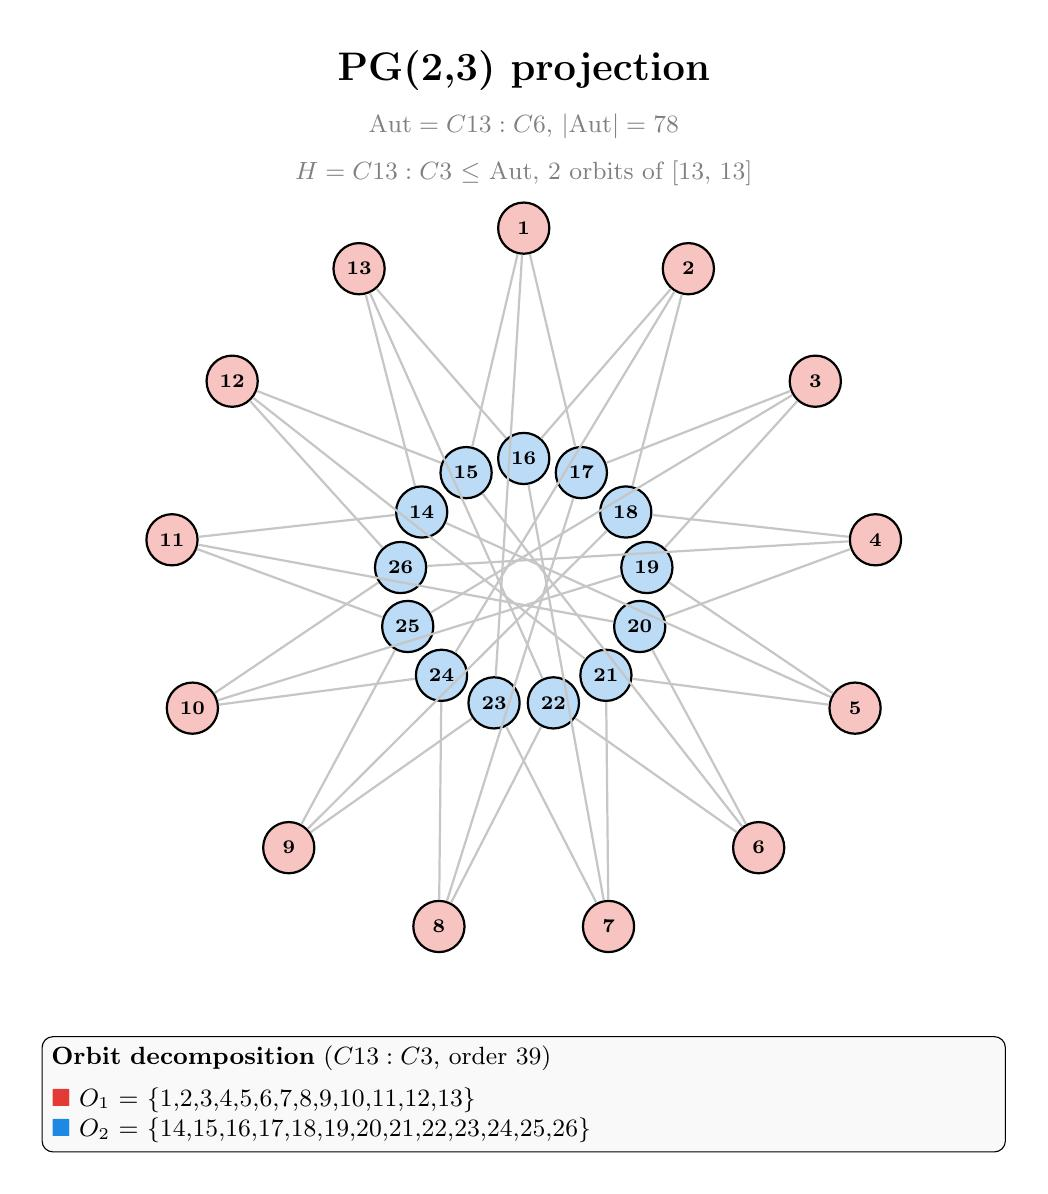
\includegraphics[width=0.92\textwidth,height=0.66\textheight,keepaspectratio]{individual_graphs/auto-pg23.jpg}
\end{center}
\vfill
Point--line incidence graph of the projective plane of order 3: $13+13 = 26$ vertices, valency 4, acted on by $\mathrm{PSL}(3,3)$. The $q=3$ sibling of the Heawood graph.

\medskip
{\small\color{gray}\texttt{individual\_graphs/auto-pg23.pdf}}
\newpage
\section{Generalized hexagon $\mathrm{GH}(2,2)$ on 63 points}
\begin{center}
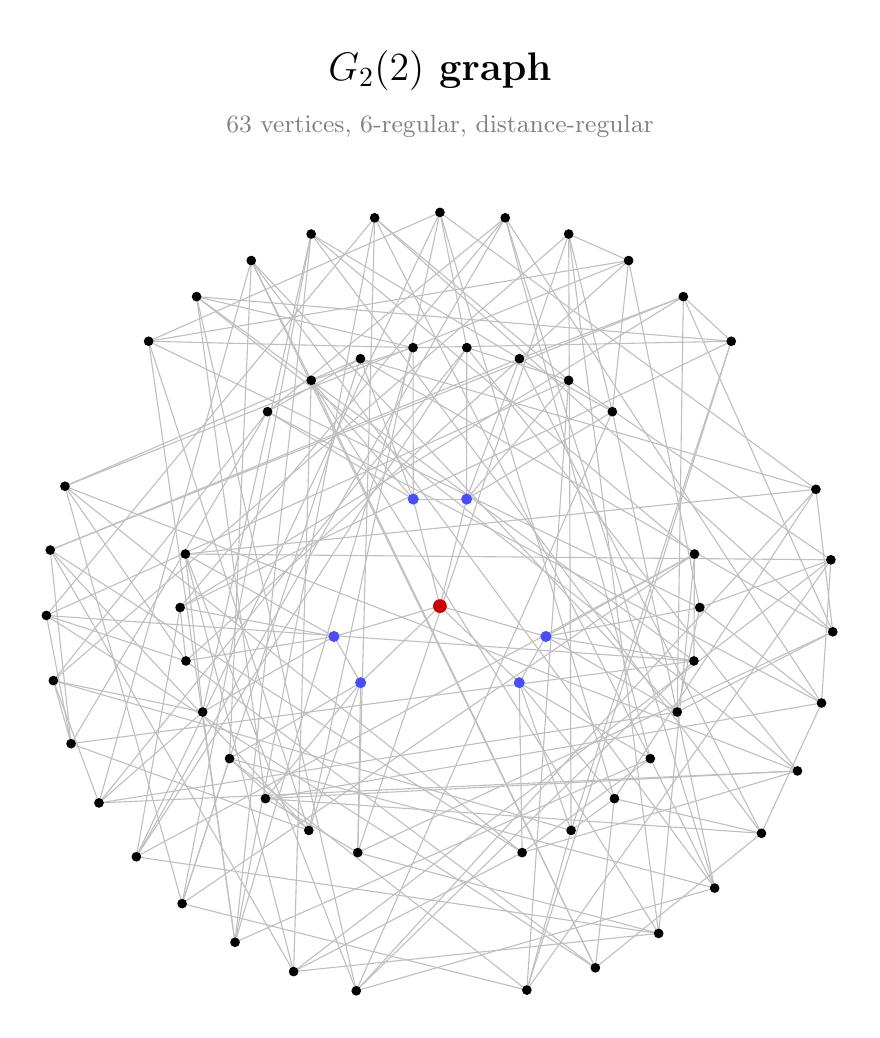
\includegraphics[width=0.92\textwidth,height=0.66\textheight,keepaspectratio]{individual_graphs/auto-gh22.jpg}
\end{center}
\vfill
Collinearity drawing of the split Cayley hexagon $\mathrm{GH}(2,2)$: the 63 points of the $G_2(2)$ hexagon with its collinearity relation. Built by src/build\_hexagon.py.

\medskip
{\small\color{gray}\texttt{individual\_graphs/auto-gh22.pdf}}
\newpage
\section{Tutte 12-cage (F126A)}
\begin{center}
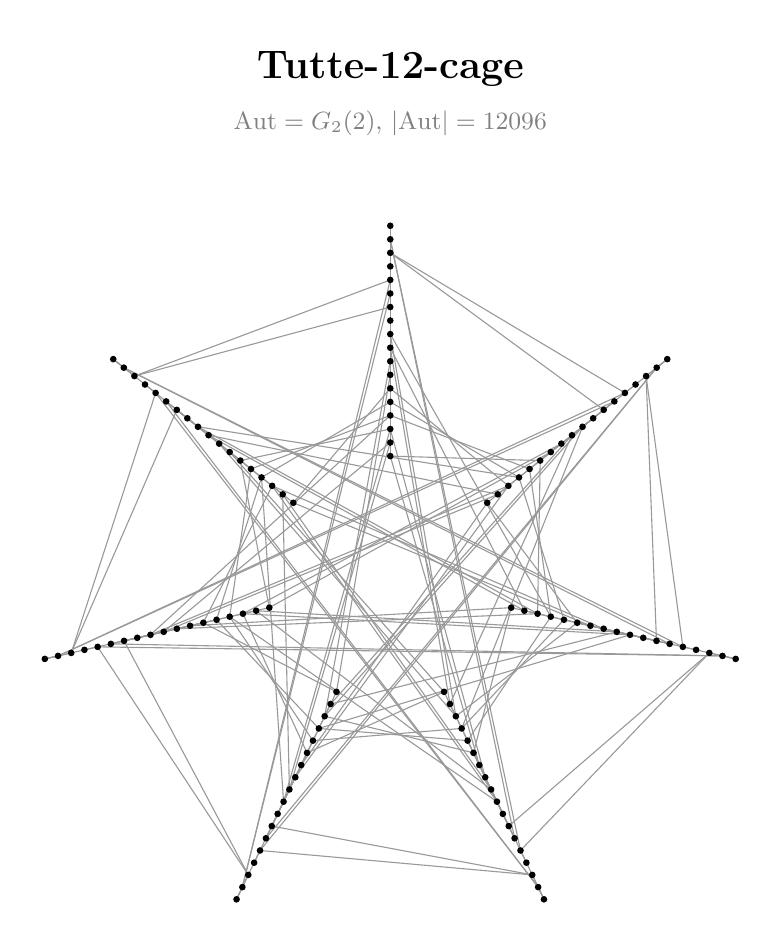
\includegraphics[width=0.92\textwidth,height=0.66\textheight,keepaspectratio]{individual_graphs/auto-tuttecage12.jpg}
\end{center}
\vfill
The Tutte 12-cage on 126 vertices: incidence graph of $\mathrm{GH}(2,2)$, $\mathrm{Aut} = G_2(2)$ of order 12096. Notably \emph{not} vertex-transitive — points and lines form orbits of $63+63$, since the hexagon is self-dual only for $q = 3^h$.

\medskip
{\small\color{gray}\texttt{individual\_graphs/auto-tuttecage12.pdf}}
\newpage
\section{Tutte 12-cage — clean rendering}
\begin{center}
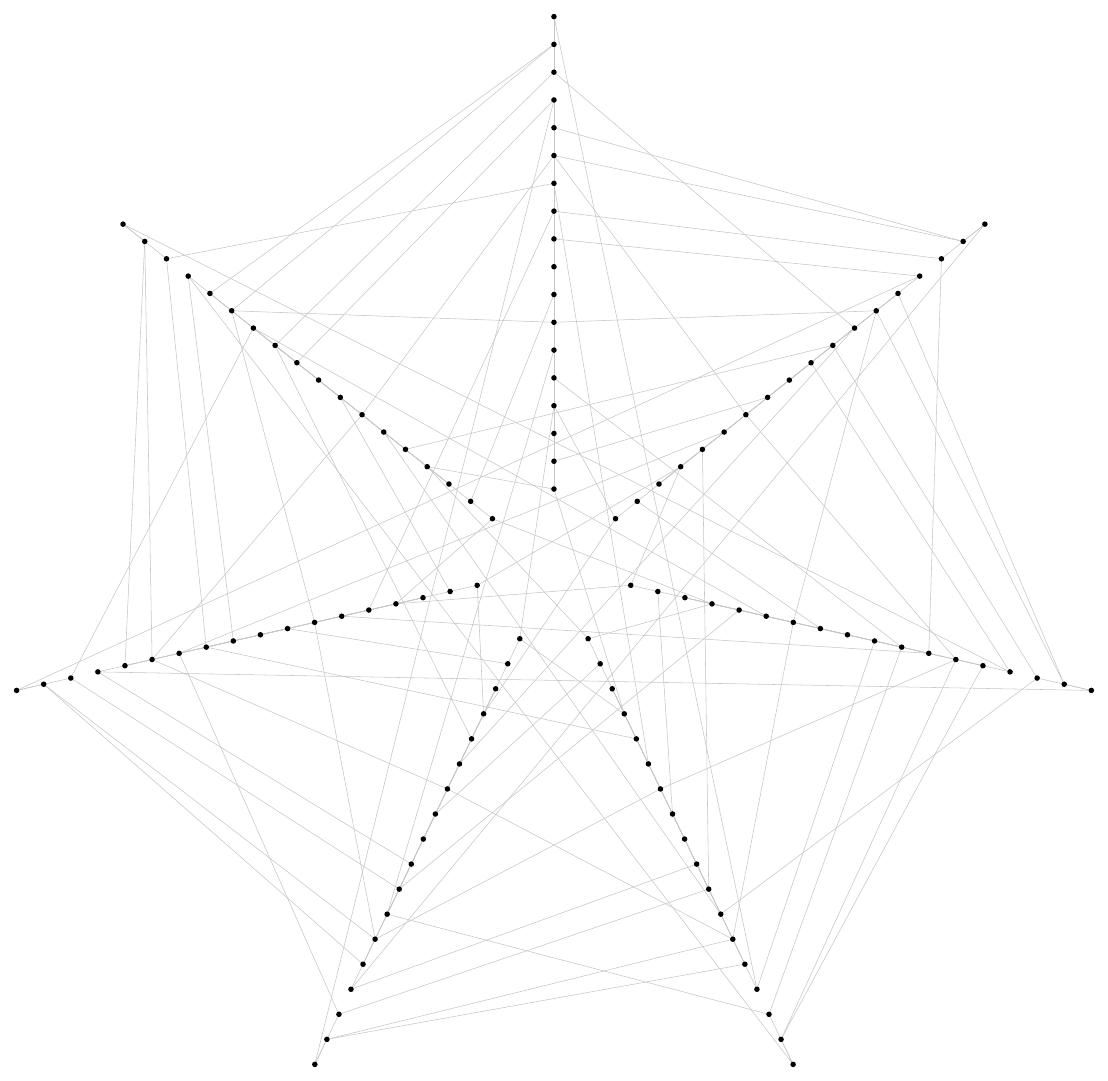
\includegraphics[width=0.92\textwidth,height=0.66\textheight,keepaspectratio]{individual_graphs/tutte12cage-clean.jpg}
\end{center}
\vfill
Hand-tuned presentation drawing of the Tutte 12-cage (labels, legend and clutter stripped) for use in papers and slides.

\medskip
{\small\color{gray}\texttt{individual\_graphs/tutte12cage-clean.pdf}}
\newpage
\section{Meinhold-72 orbital graph}
\begin{center}
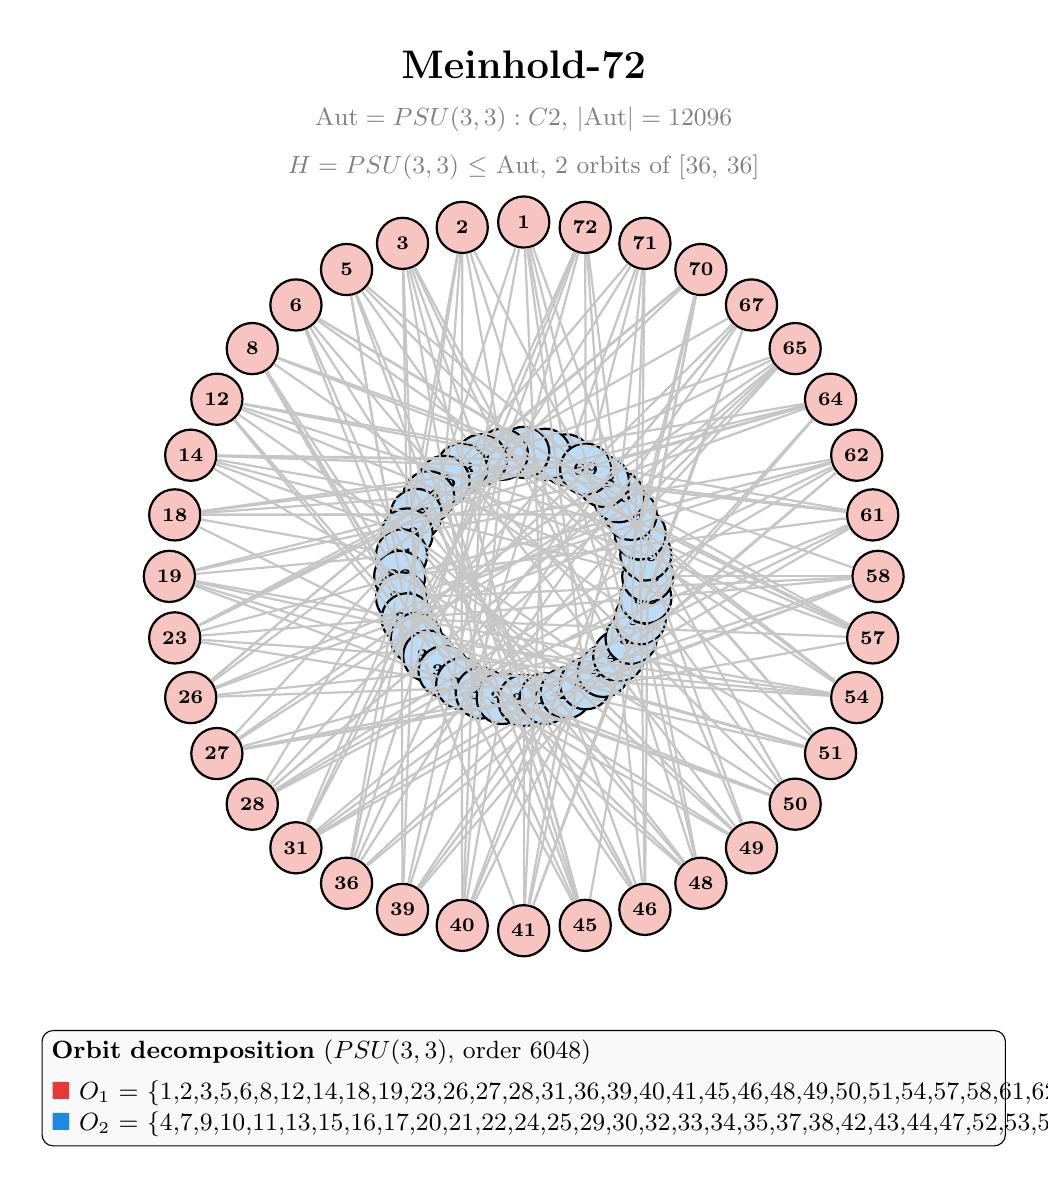
\includegraphics[width=0.92\textwidth,height=0.66\textheight,keepaspectratio]{individual_graphs/auto-meinhold72.jpg}
\end{center}
\vfill
Orbital graph of $G_2(2)$ acting on the 72 cosets of $\mathrm{PSL}(3,2)$. Its rank-8 Hecke algebra satisfies $B^2 = 13I$ — the ``why 13'' story ($13 = 7 + 2\cdot 3$ via the 36+36 chiral Fano structures); see the why13 paper in the hecke repo.

\medskip
{\small\color{gray}\texttt{individual\_graphs/auto-meinhold72.pdf}}
\newpage
\section{$F_{056A}$}
\begin{center}
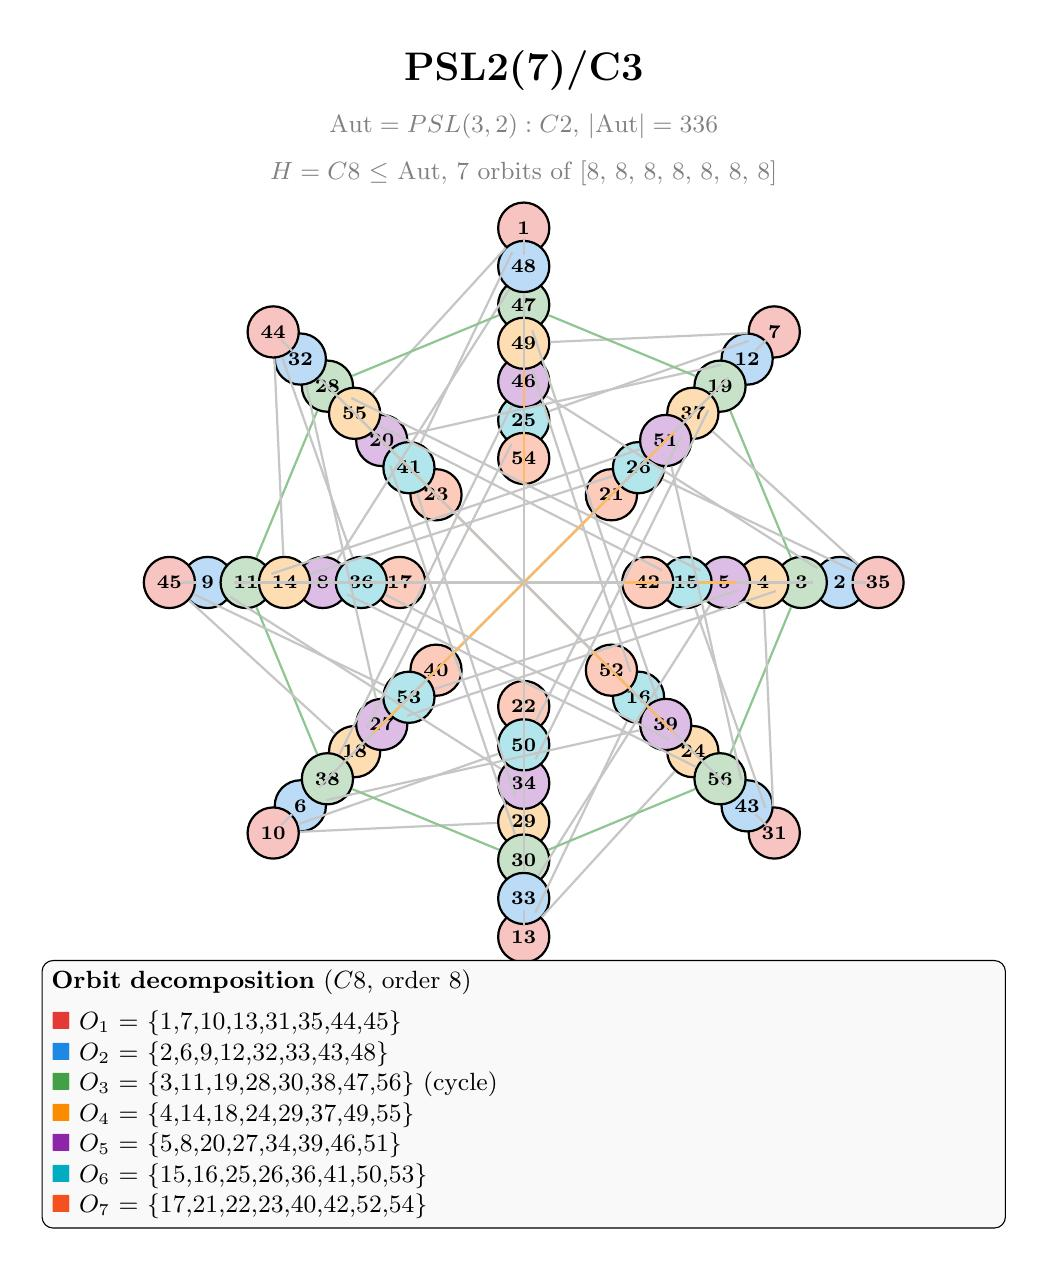
\includegraphics[width=0.92\textwidth,height=0.66\textheight,keepaspectratio]{individual_graphs/F056A.jpg}
\end{center}
\vfill
The Foster-census graph F056A on 56 vertices, cubic arc-transitive.

\medskip
{\small\color{gray}\texttt{individual\_graphs/F056A.pdf}}
\newpage
\section{$F_{056A}$ — minimal rendering}
\begin{center}
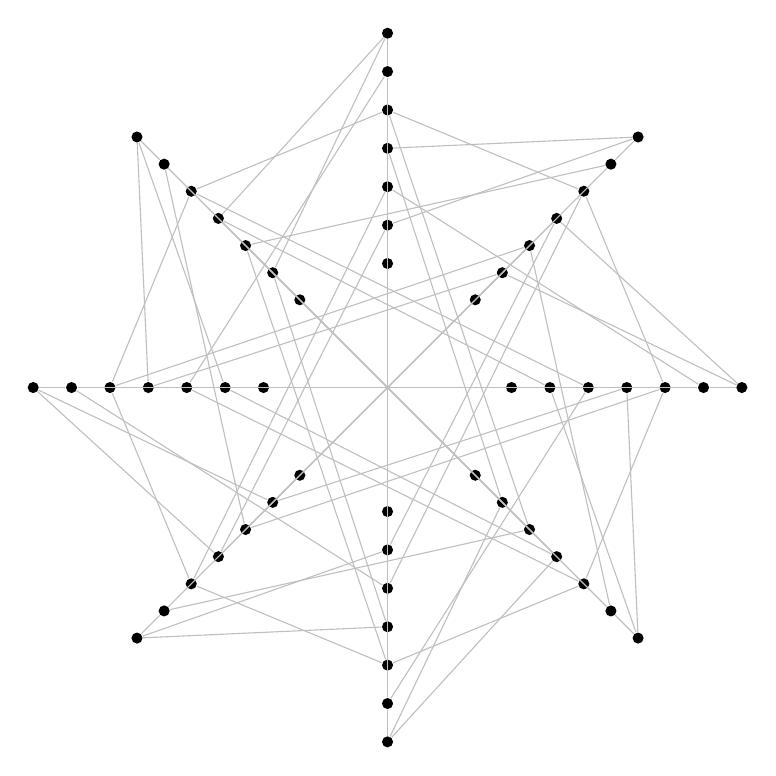
\includegraphics[width=0.92\textwidth,height=0.66\textheight,keepaspectratio]{individual_graphs/F056A-minimal.jpg}
\end{center}
\vfill
Hand-edited minimal drawing of F056A, decluttered for presentation.

\medskip
{\small\color{gray}\texttt{individual\_graphs/F056A-minimal.pdf}}
\newpage
\addtocontents{toc}{\protect\vspace{0.5em}\protect\noindent\textbf{Voltage Graphs \& Variants}\protect\par}
\section{Petersen — voltage graph construction}
\begin{center}
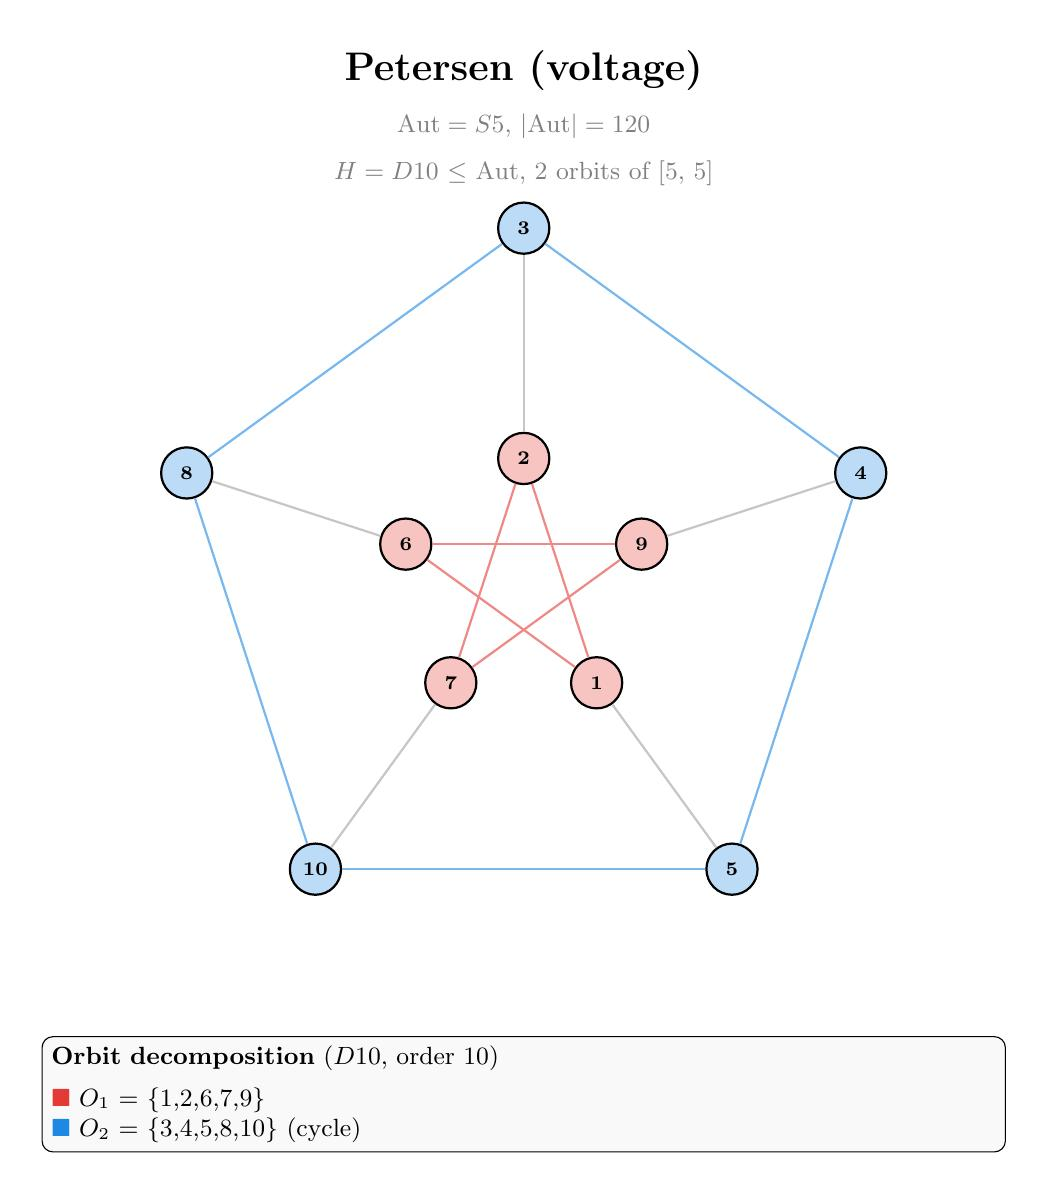
\includegraphics[width=0.92\textwidth,height=0.66\textheight,keepaspectratio]{individual_graphs/auto-petersen_voltage.jpg}
\end{center}
\vfill
The Petersen graph presented as a voltage graph: the base quotient with $\mathbb{Z}_5$ voltage labels whose derived graph reconstructs the full graph.

\medskip
{\small\color{gray}\texttt{individual\_graphs/auto-petersen\_voltage.pdf}}
\newpage
\section{Heawood — voltage graph construction}
\begin{center}
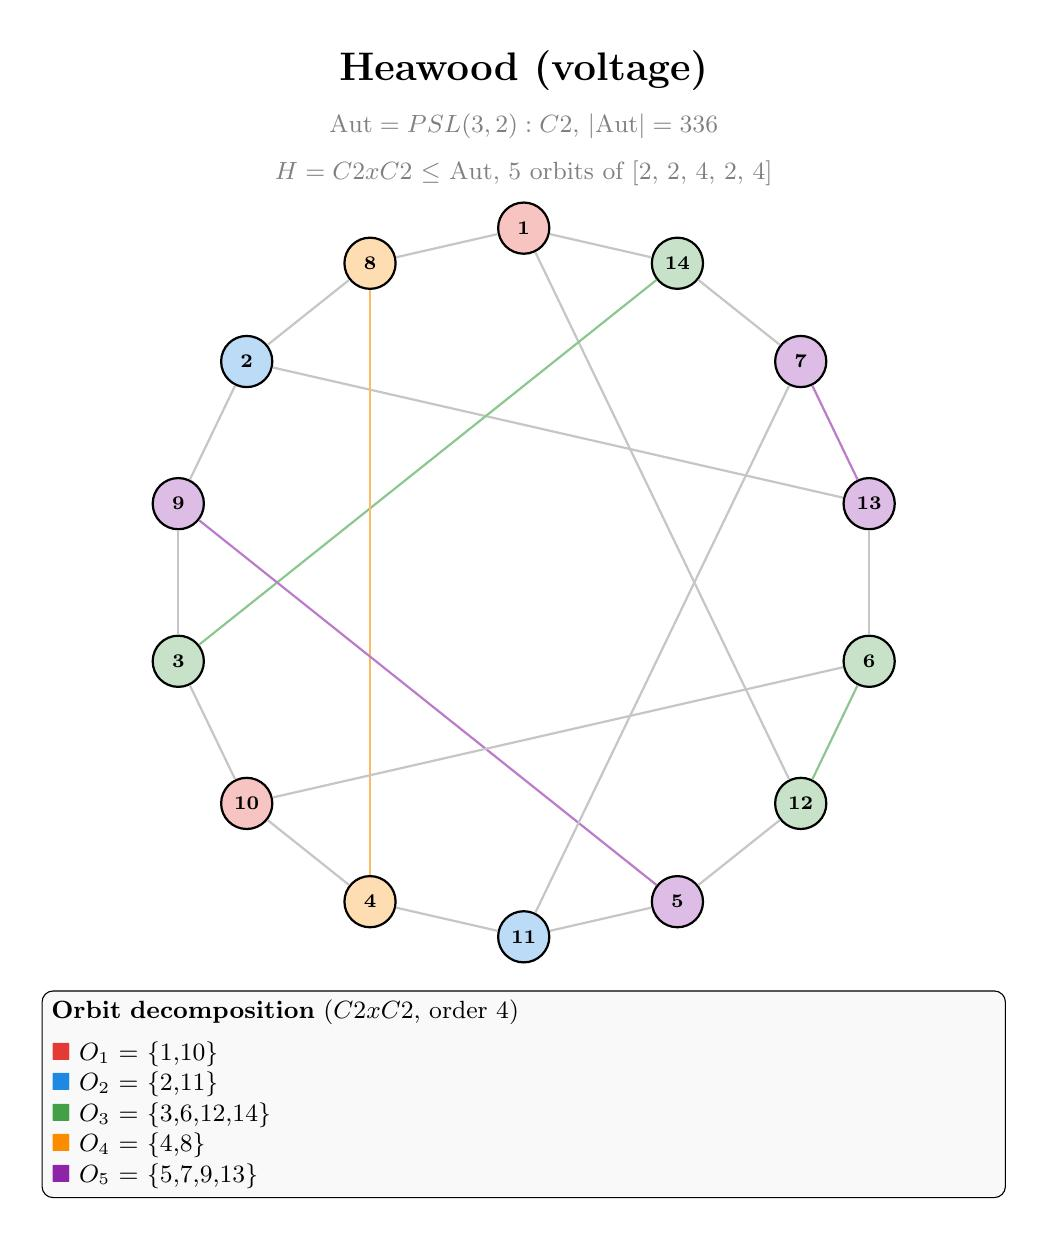
\includegraphics[width=0.92\textwidth,height=0.66\textheight,keepaspectratio]{individual_graphs/auto-heawood_voltage.jpg}
\end{center}
\vfill
Voltage-graph presentation of the Heawood graph: a small quotient with cyclic voltage labels encoding the 14-vertex cover.

\medskip
{\small\color{gray}\texttt{individual\_graphs/auto-heawood\_voltage.pdf}}
\newpage
\section{M\"obius--Kantor — voltage graph construction}
\begin{center}
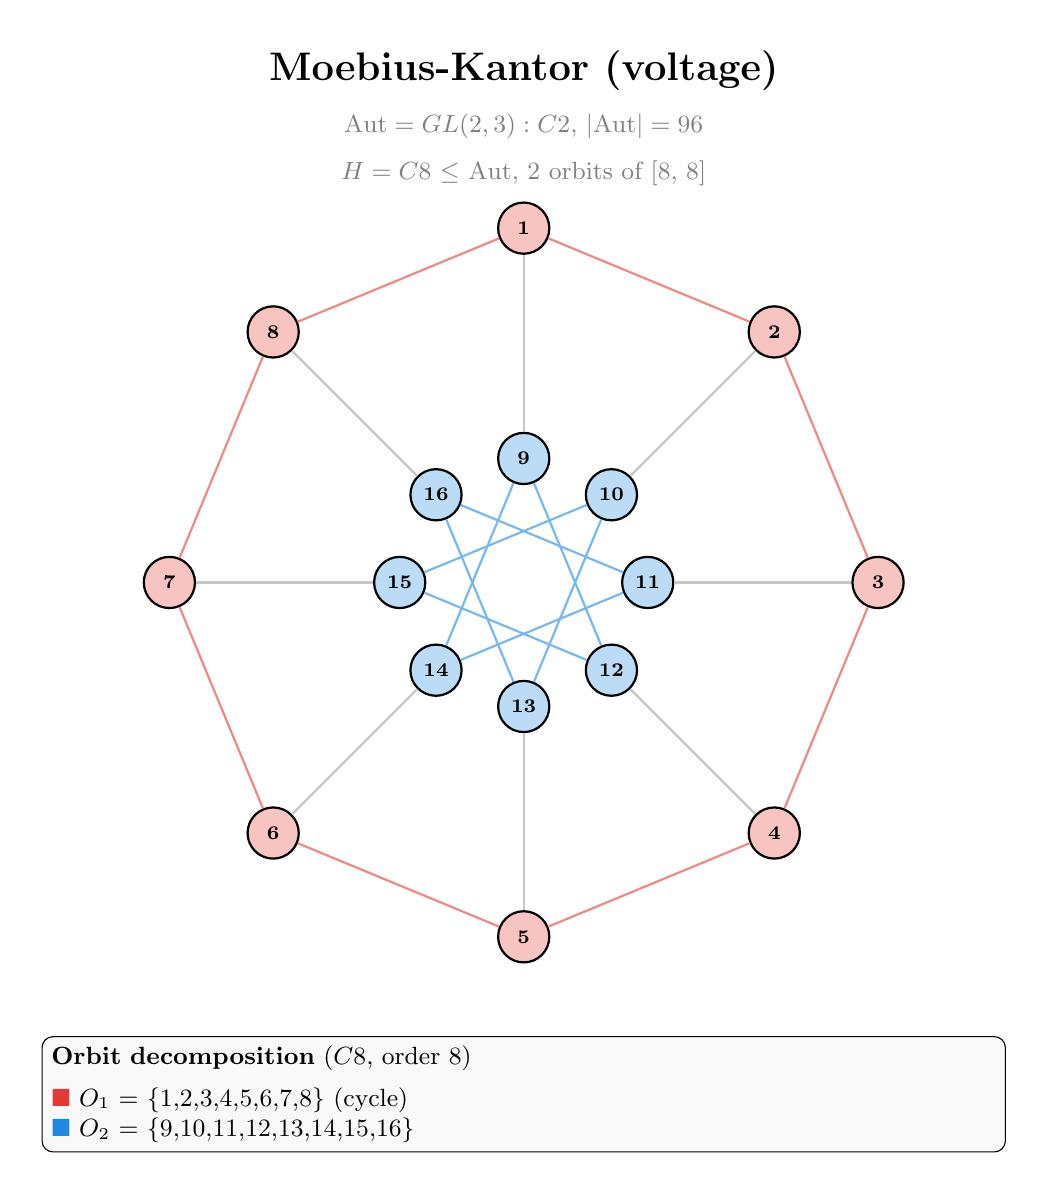
\includegraphics[width=0.92\textwidth,height=0.66\textheight,keepaspectratio]{individual_graphs/auto-mk_voltage.jpg}
\end{center}
\vfill
Voltage-graph presentation of the M\"obius--Kantor graph $\mathrm{GP}(8,3)$.

\medskip
{\small\color{gray}\texttt{individual\_graphs/auto-mk\_voltage.pdf}}
\newpage
\section{Tutte--Coxeter — clean rendering}
\begin{center}
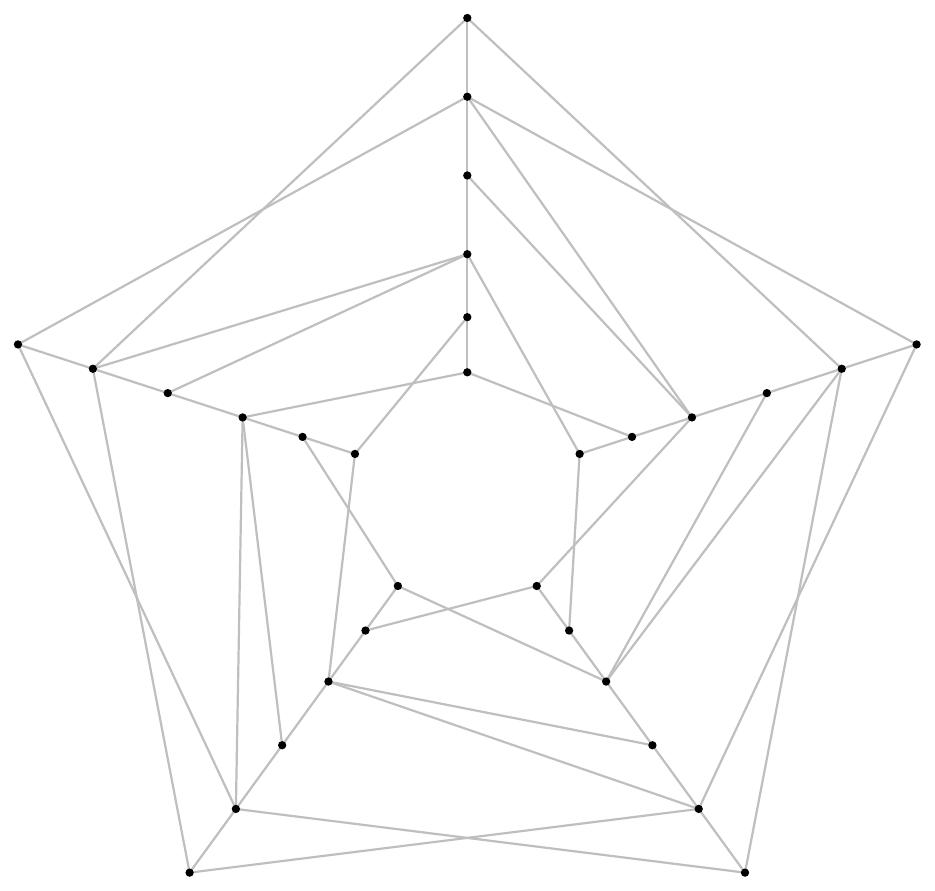
\includegraphics[width=0.92\textwidth,height=0.66\textheight,keepaspectratio]{individual_graphs/tuttecoxeter-clean.jpg}
\end{center}
\vfill
Hand-tuned presentation drawing of the Tutte--Coxeter graph (F030A, the $(3,8)$-cage).

\medskip
{\small\color{gray}\texttt{individual\_graphs/tuttecoxeter-clean.pdf}}
\newpage
\section{Cage pair}
\begin{center}
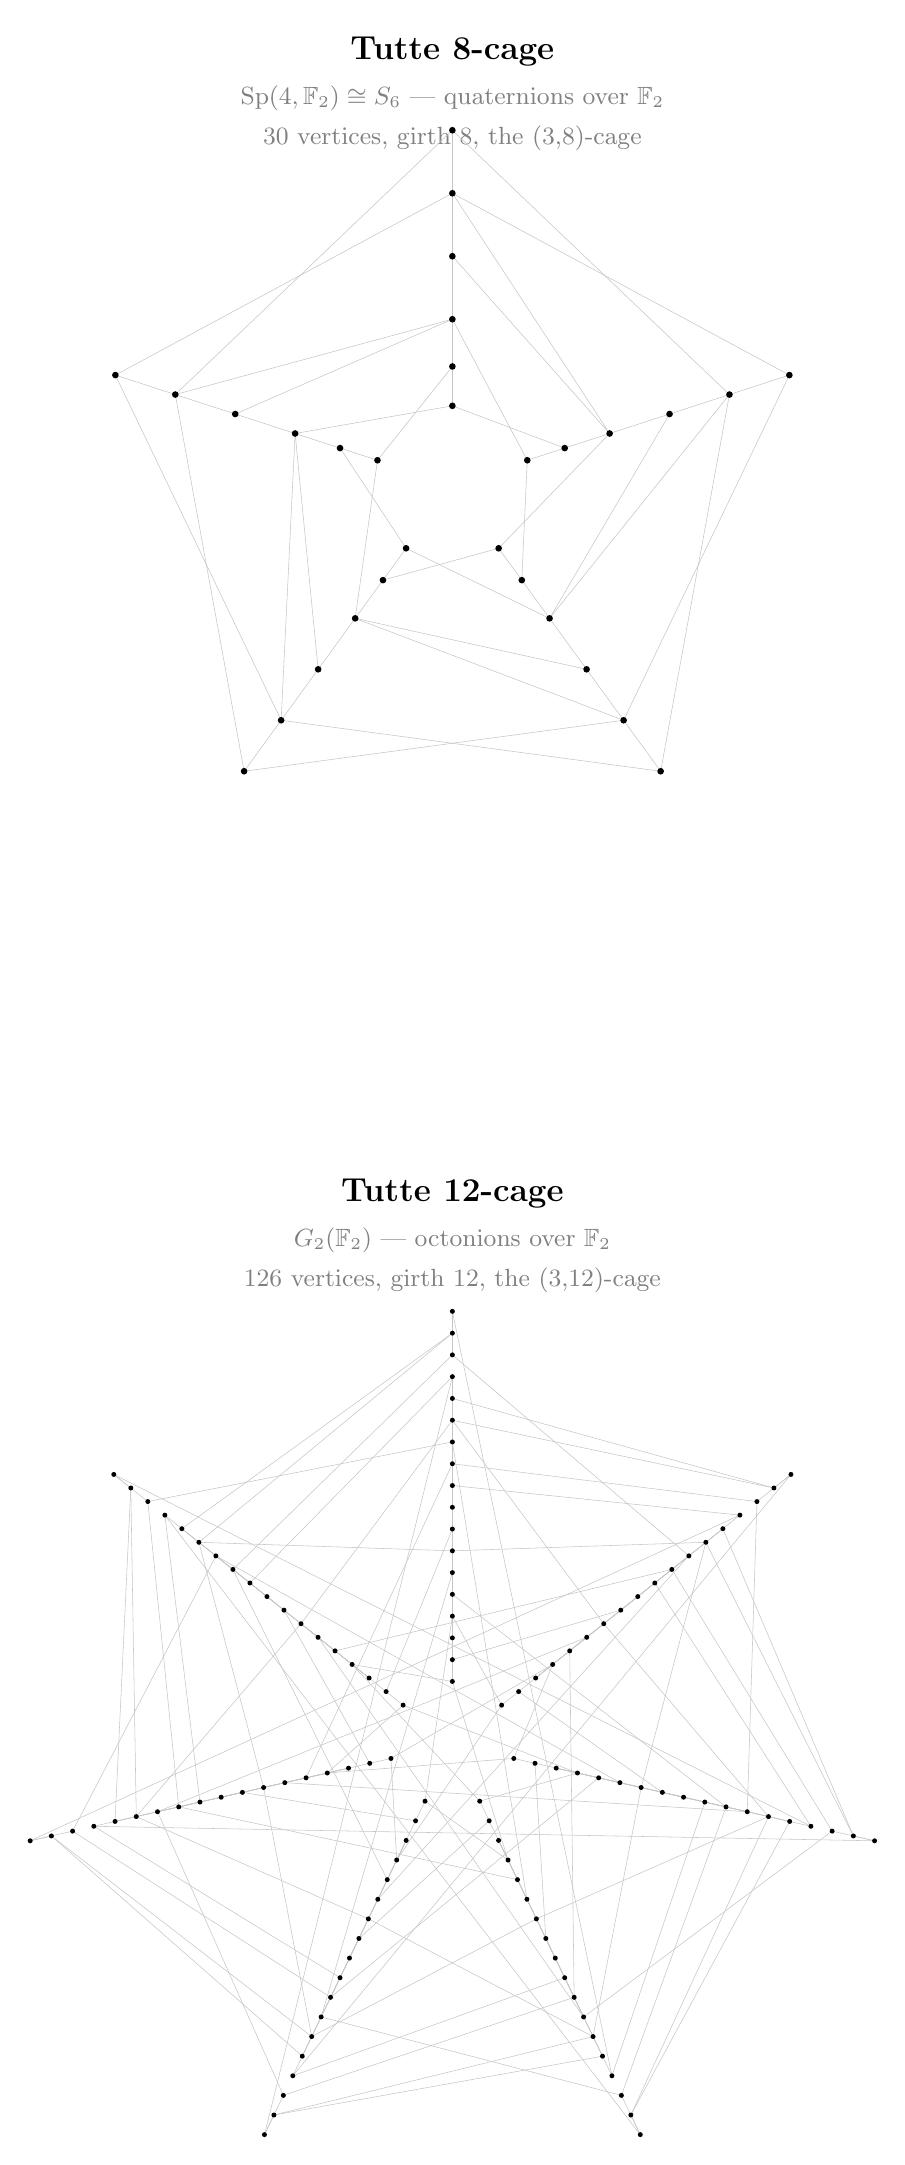
\includegraphics[width=0.92\textwidth,height=0.66\textheight,keepaspectratio]{individual_graphs/cage-pair.jpg}
\end{center}
\vfill
Hand-edited side-by-side of two cages from the generalized-polygon series at $s=2$: the $(3,8)$-cage (Tutte--Coxeter, $\mathrm{GQ}(2,2)$) and the $(3,12)$-cage (Tutte 12-cage, $\mathrm{GH}(2,2)$).

\medskip
{\small\color{gray}\texttt{individual\_graphs/cage-pair.pdf}}
\newpage
\addtocontents{toc}{\protect\vspace{0.5em}\protect\noindent\textbf{Klein Quartic \& Quotients}\protect\par}
\section{Klein quartic graph — $C_7$ layout}
\begin{center}
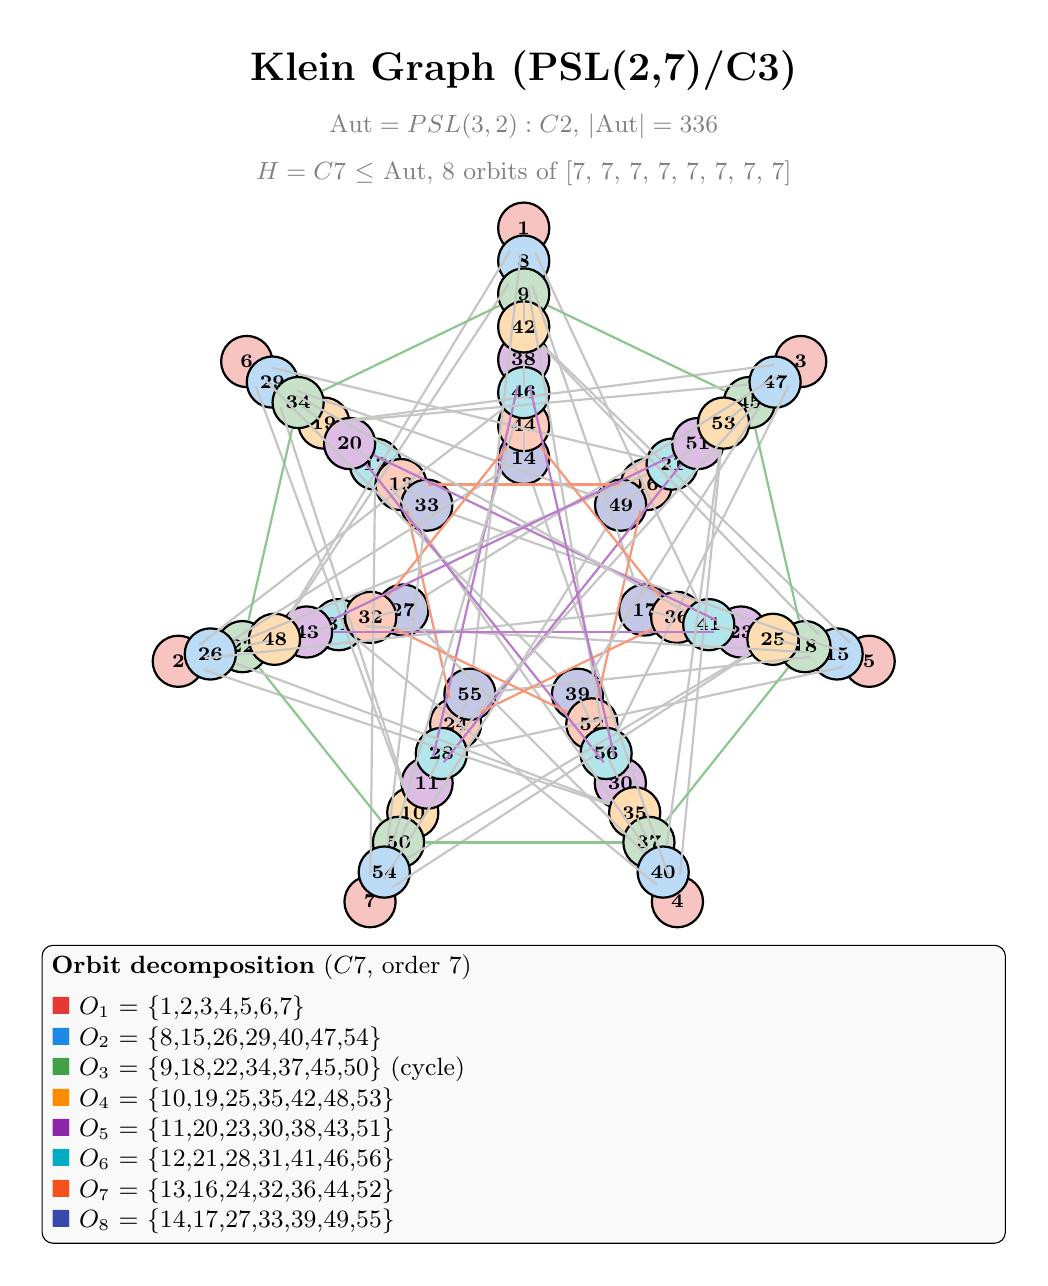
\includegraphics[width=0.92\textwidth,height=0.66\textheight,keepaspectratio]{individual_graphs/auto-klein-c7.jpg}
\end{center}
\vfill
Graph derived from the Klein quartic's $\mathrm{PSL}(2,7)$ cell structure (genus 3, Hurwitz-maximal with 168 automorphisms), laid out on $C_7$ orbit rings.

\medskip
{\small\color{gray}\texttt{individual\_graphs/auto-klein-c7.pdf}}
\newpage
\section{Klein quartic graph — minimal rendering}
\begin{center}
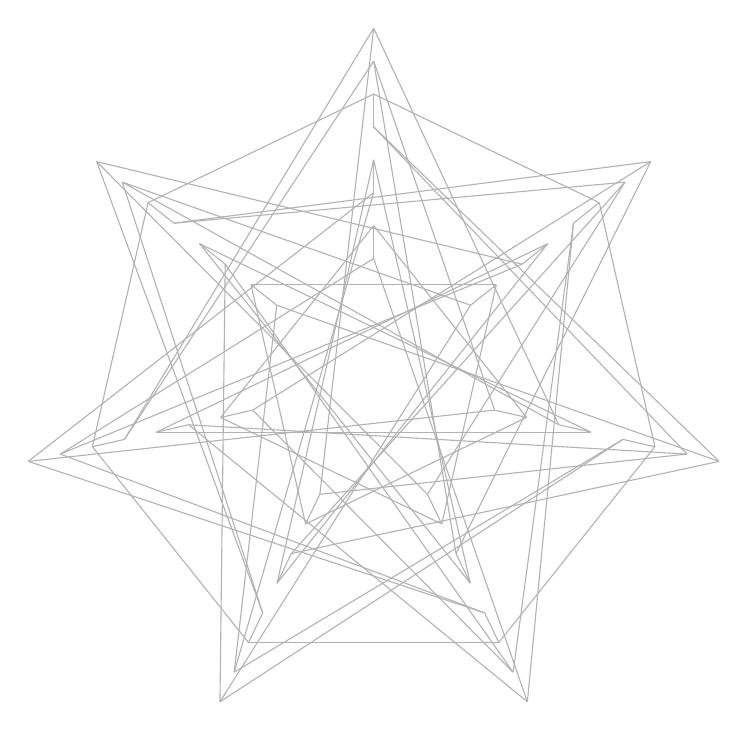
\includegraphics[width=0.92\textwidth,height=0.66\textheight,keepaspectratio]{individual_graphs/auto-klein-minimal.jpg}
\end{center}
\vfill
Decluttered drawing of the Klein quartic graph.

\medskip
{\small\color{gray}\texttt{individual\_graphs/auto-klein-minimal.pdf}}
\newpage
\section{Klein graph — $\mathbb{Z}_2$ quotient}
\begin{center}
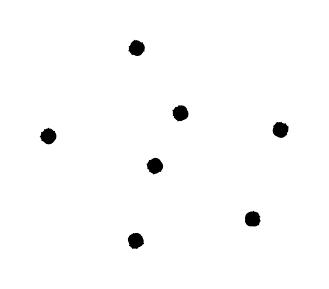
\includegraphics[width=0.92\textwidth,height=0.66\textheight,keepaspectratio]{individual_graphs/klein-z2-quotient.jpg}
\end{center}
\vfill
Hand-edited drawing of a $\mathbb{Z}_2$ quotient of the Klein quartic graph, from the quotient-surfaces side-programme.

\medskip
{\small\color{gray}\texttt{individual\_graphs/klein-z2-quotient.pdf}}
\newpage
\section{Zhou $\mathbb{Z}_2$-quotient}
\begin{center}
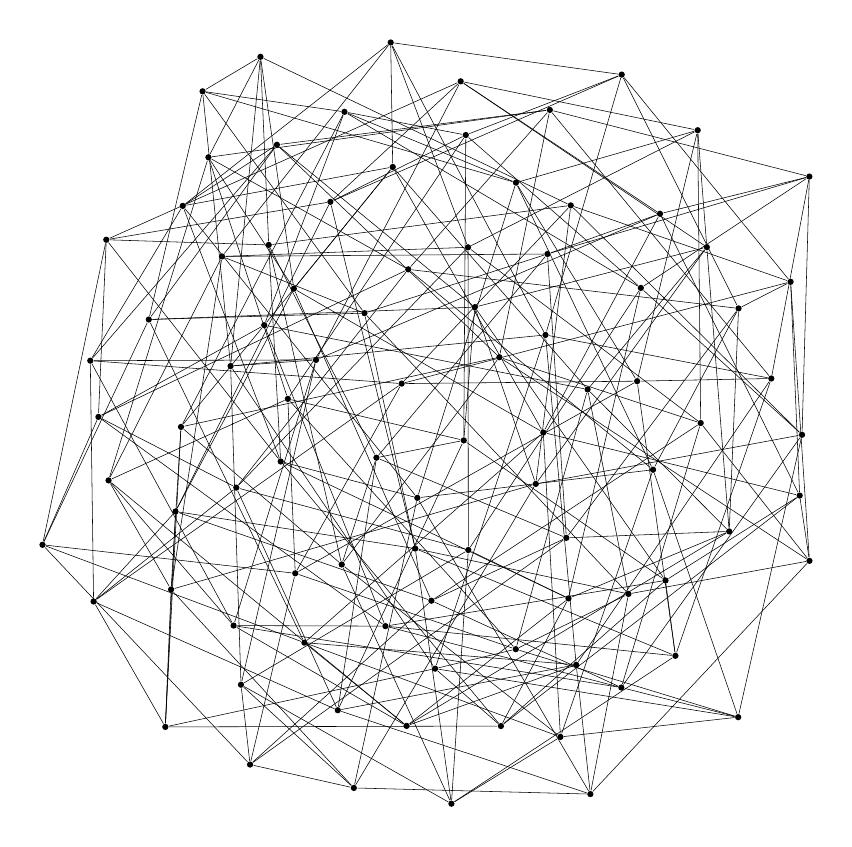
\includegraphics[width=0.92\textwidth,height=0.66\textheight,keepaspectratio]{individual_graphs/zhou-z2-quotient.jpg}
\end{center}
\vfill
The Zhou $\mathbb{Z}_2$-quotient construction from the clayworth CSS-code programme (quotients of graph tilings yielding quantum error-correcting codes).

\medskip
{\small\color{gray}\texttt{individual\_graphs/zhou-z2-quotient.pdf}}
\newpage
\section{Zhou quotient — spectral layout}
\begin{center}
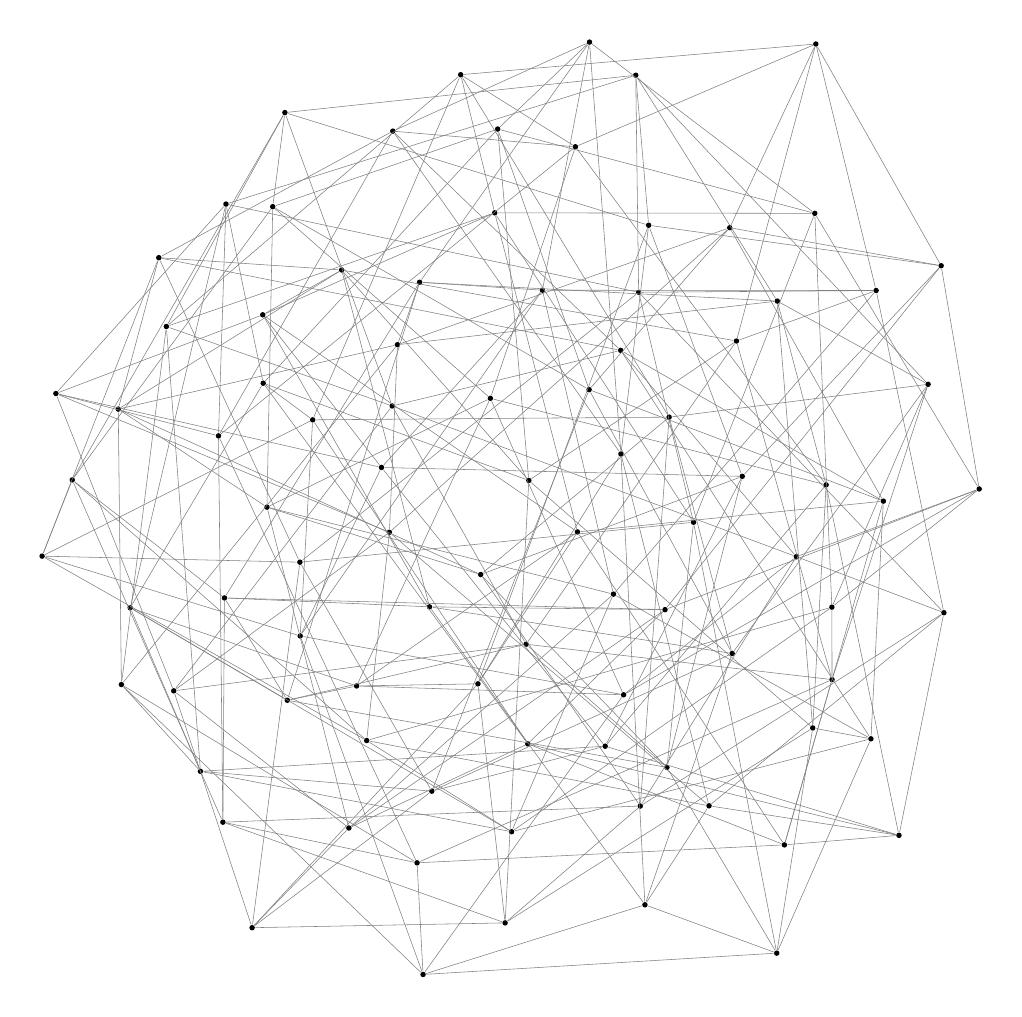
\includegraphics[width=0.92\textwidth,height=0.66\textheight,keepaspectratio]{individual_graphs/zhou-quotient-spectral.jpg}
\end{center}
\vfill
The same Zhou quotient drawn with a spectral (eigenvector) layout for comparison with the orbit-ring method.

\medskip
{\small\color{gray}\texttt{individual\_graphs/zhou-quotient-spectral.pdf}}
\newpage
\end{document}
